% !TEX program = xelatex

\documentclass[aspectratio=169]{beamer}

\usetheme{metropolis}
\setbeamerfont{frametitle}{size=\small}
\setbeamerfont{normal text}{size=\small}
\setbeamerfont{section title}{size=\small}
\setbeamerfont{title}{size=\small}
\usefonttheme[onlymath]{serif}
\setbeamertemplate{footline}{}

\makeatletter
\setbeamertemplate{frametitle continuation}{(\insertcontinuationcount)}

\makeatother

\setlength{\abovedisplayskip}{0pt}
\setlength{\belowdisplayskip}{4pt}

\usepackage{fontspec}
\usepackage{graphicx}
\usepackage{amsmath}
\usepackage{etoolbox}
\usepackage[orientation=landscape,size=custom,width=16,height=9,scale=0.5,debug]{beamerposter} 

\setlength{\jot}{0pt}

\renewcommand{\baselinestretch}{0.95}

\title{Методы понижения размерности данных}
\author{Поглазов Никита}
\date{2024}

\begin{document}

\maketitle

\section{Введение}
\begin{frame}{Введение}
    \textbf{Проклятие размерности:} данные высокой размерности сложны для анализа, требуют много вычислительных ресурсов и часто содержат шум.

    \begin{figure}
        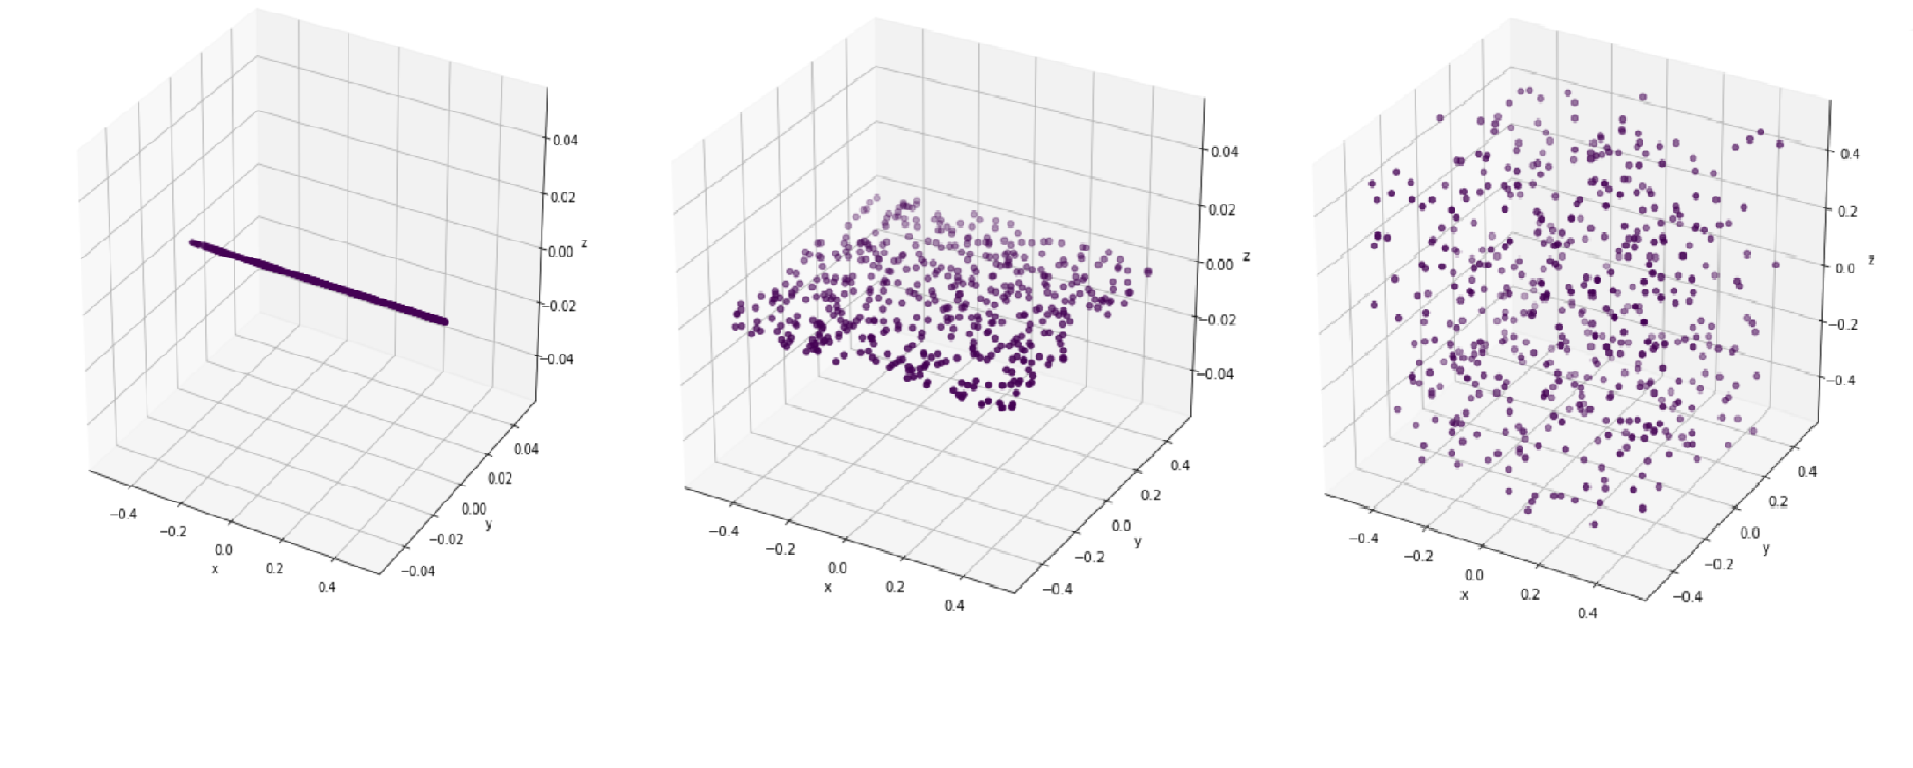
\includegraphics[width=.7 \textwidth]{../resources/intro/dim_curse.png}
    \end{figure}
\end{frame}

\section{Мотивация}

\begin{frame}{Что такое "проклятие размерности"?}
    $$
        S_{square}=1 \quad S_{circle}=\pi*(0.5)^2=\frac{\pi}{4}\approx0.79
    $$
    \begin{figure}
        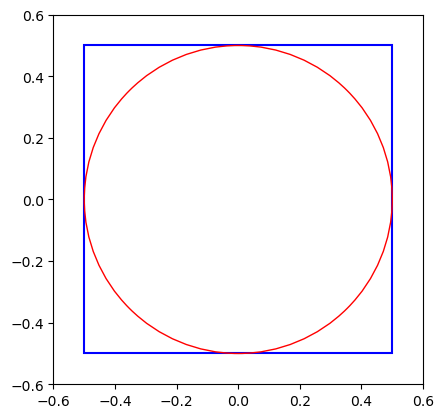
\includegraphics[width=0.6\textwidth]{../resources/motivation/inscribed_circle.png}
    \end{figure}
\end{frame}

\begin{frame}{Гиперсфера и гиперкуб}
    \begin{itemize}
        \item Объем гиперсферы стремится к нулю при росте размерности:
              \begin{equation*}
                  V_n = \frac{\pi^{n/2}}{\Gamma(\frac{n}{2}+1)}R^n
              \end{equation*}
        \item Диагональ гиперкуба увеличивается как \(\sqrt{n}\).
    \end{itemize}
    \begin{figure}
        \centering
        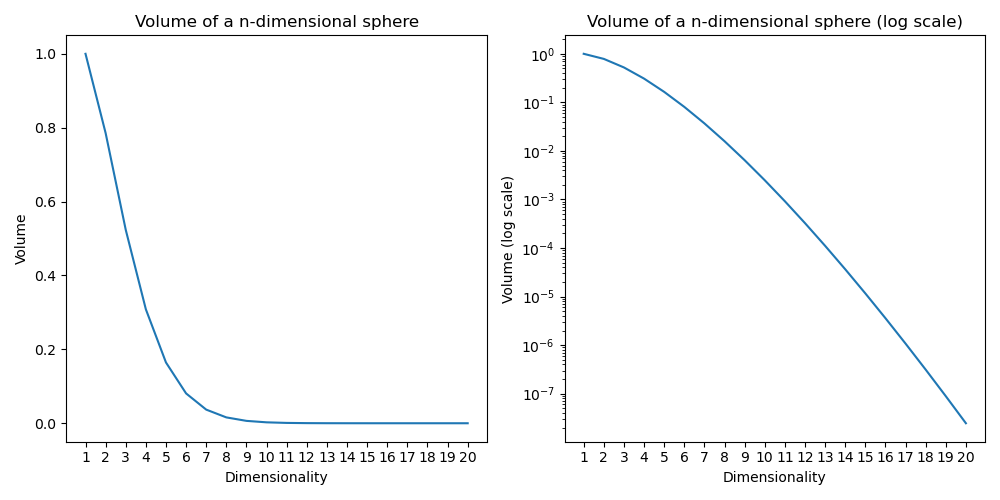
\includegraphics[width=0.7\textwidth]{../resources/motivation/sphere_volume.png}
    \end{figure}
\end{frame}

\begin{frame}[allowframebreaks]{Влияние на метрические модели}
    \begin{itemize}
        \item Манхэттенское расстояние:
              \begin{equation*}
                  d(x^{(i)}, x^{(j)}) = \sum_{k=1}^n |x_k^{(i)} - x_k^{(j)}|
              \end{equation*}
        \item Средние расстояния между точками становятся близкими:
              \begin{equation*}
                  \lim_{n\to\infty}\frac{d(x^{(i)}, x^{(j)})}{n} = \mu
              \end{equation*}
        \item Сохраняется и для $L_2$ нормы.
    \end{itemize}
    
    \begin{figure}
        \centering
        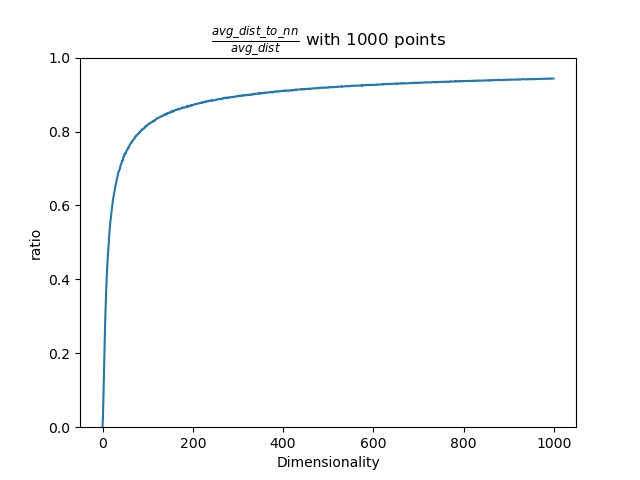
\includegraphics[width=.7\textwidth]{../resources/motivation/ratio.png}
    \end{figure}
\end{frame}

\begin{frame}{Линейная регрессия и мультиколлинеарность}
    \begin{itemize}
        \item Решение задачи MSE:
              \begin{equation*}
                  (X^TX)\hat{\beta} = X^Ty
              \end{equation*}
        \item Матричная ковариация:
              \begin{equation*}
                  \mathrm{Cov}(X) = \frac{1}{k-1}X^TX
              \end{equation*}
        \item Высокая корреляция между признаками \(\Rightarrow\) нестабильные веса, переобучение.
    \end{itemize}
\end{frame}

\begin{frame}{Влияние на "деревянные" модели}
    \begin{itemize}
        \item Сложность выбора оптимального разделения при высокой размерности.
        \item Деревья склонны к переобучению из-за случайных разбиений.
        \item \textbf{Workaround:} \textit{Random Subspace Method} (Но)
    \end{itemize}
\end{frame}

\begin{frame}{Влияние на глубокие нейронные сети}
    \begin{itemize}
        \item Сверточные сети (\textit{CNN}) используют локальные взаимосвязи.
        \item \textit{LSTM} моделируют временные зависимости, игнорируя пространственные.
        \item Трансформеры извлекают только значимые зависимости.
        \item Проблемы: обучение на шуме, сложность оптимизации функционала потерь.
    \end{itemize}
\end{frame}

\begin{frame}{Общее влияние "проклятия размерности"}
    \begin{itemize}
        \item Увеличение времени обучения моделей.
        \item Сложность интерпретации табличных данных.
        \item Вероятность обучения на шумовых признаках \(\Rightarrow\) переобучение.
    \end{itemize}
\end{frame}
\section{Обзор и классификация методов}

\begin{frame}{Два подхода к понижению размерности}
    \textbf{Отбор признаков:}
    \begin{itemize}
        \item Выбор подмножества исходных признаков.
        \item Сохранение информации без преобразования данных.
    \end{itemize}

    \textbf{Преобразование признаков:}
    \begin{itemize}
        \item Трансформация данных в новое пространство меньшей размерности.
        \item Сохраняет наиболее значимые свойства данных.
    \end{itemize}

    \begin{figure}
        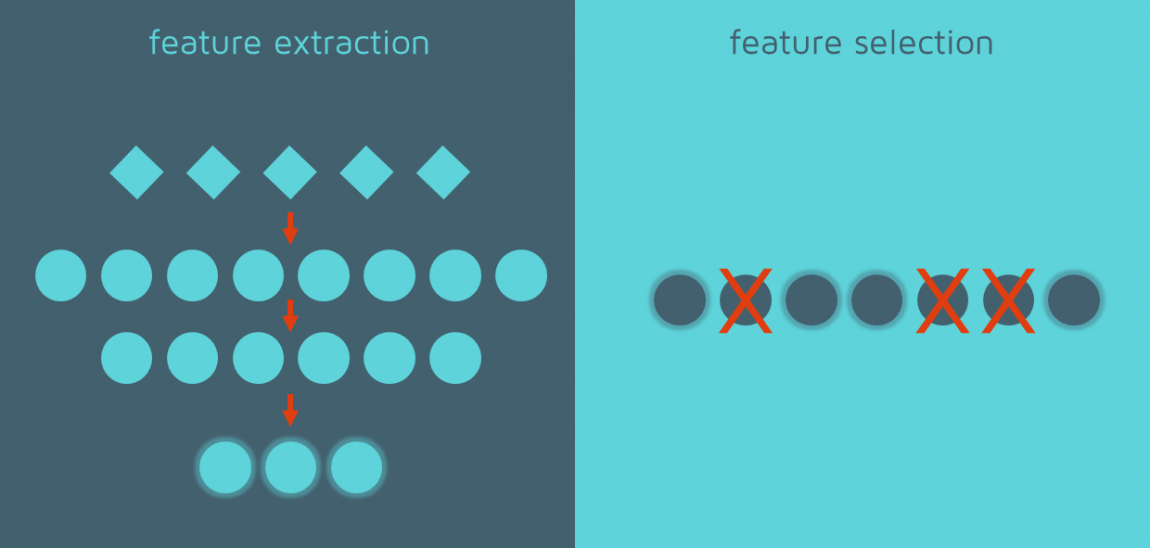
\includegraphics[width=.5\textwidth]{../resources/methods/feature_selection_vs_extraction.png}
    \end{figure}
\end{frame}

\begin{frame}
    \frametitle{Линейные методы}
    \begin{columns}
        \column{.6\textwidth}
        \begin{itemize}
            \item Предполагают, что данные лежат в \textbf{линейном подпространстве}.
            \item Преобразуют данные с помощью \textbf{линейных операций}.
        \end{itemize}
        \column{.6\textwidth}
        \begin{center}
            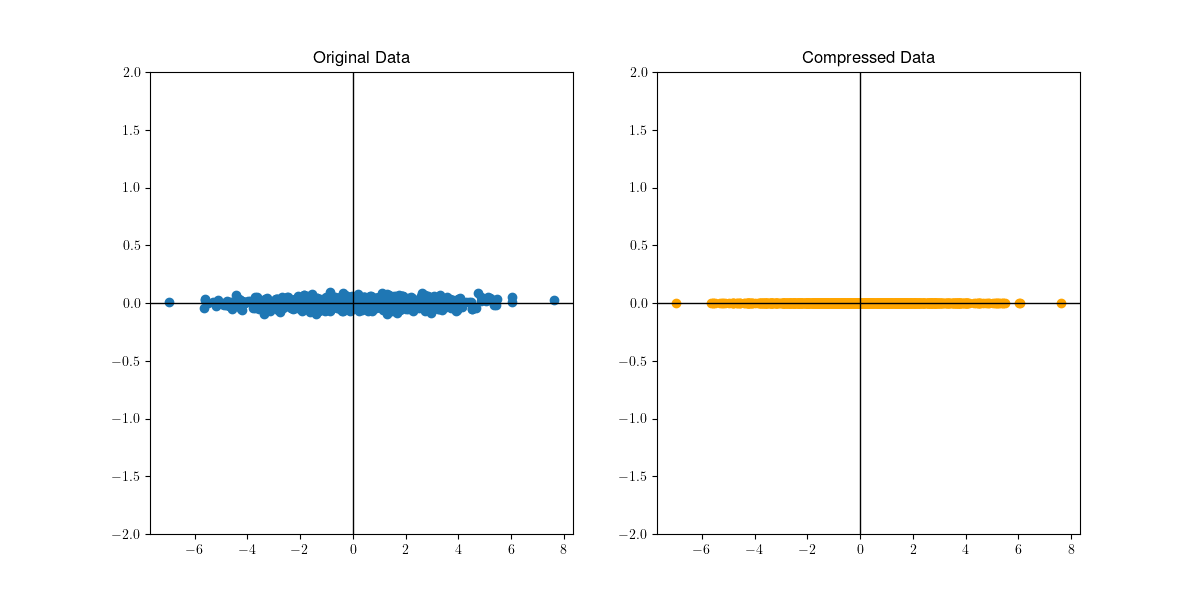
\includegraphics[width=.9\textwidth]{../resources/pca/simple_example_both.png}
            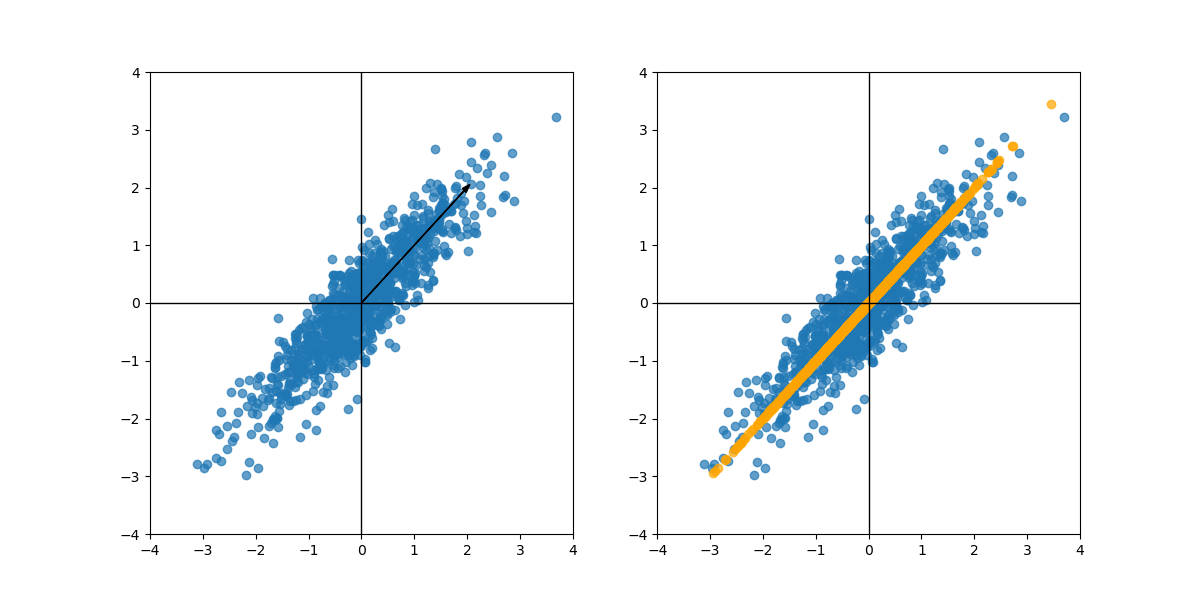
\includegraphics[width=.9\textwidth]{../resources/methods/pca.png}
        \end{center}
    \end{columns}
\end{frame}

\begin{frame}
    \frametitle{Нелинейные методы}
    \begin{columns}
        \column{0.55\textwidth}
        \begin{itemize}
            \item Данные имеют \textbf{сложные взаимосвязи}, которые нельзя описать линейно.
            \item Методы выявляют \textbf{нелинейные структуры} и сворачивают их в более простую форму.
        \end{itemize}
        \column{0.55\textwidth}
        \begin{center}
            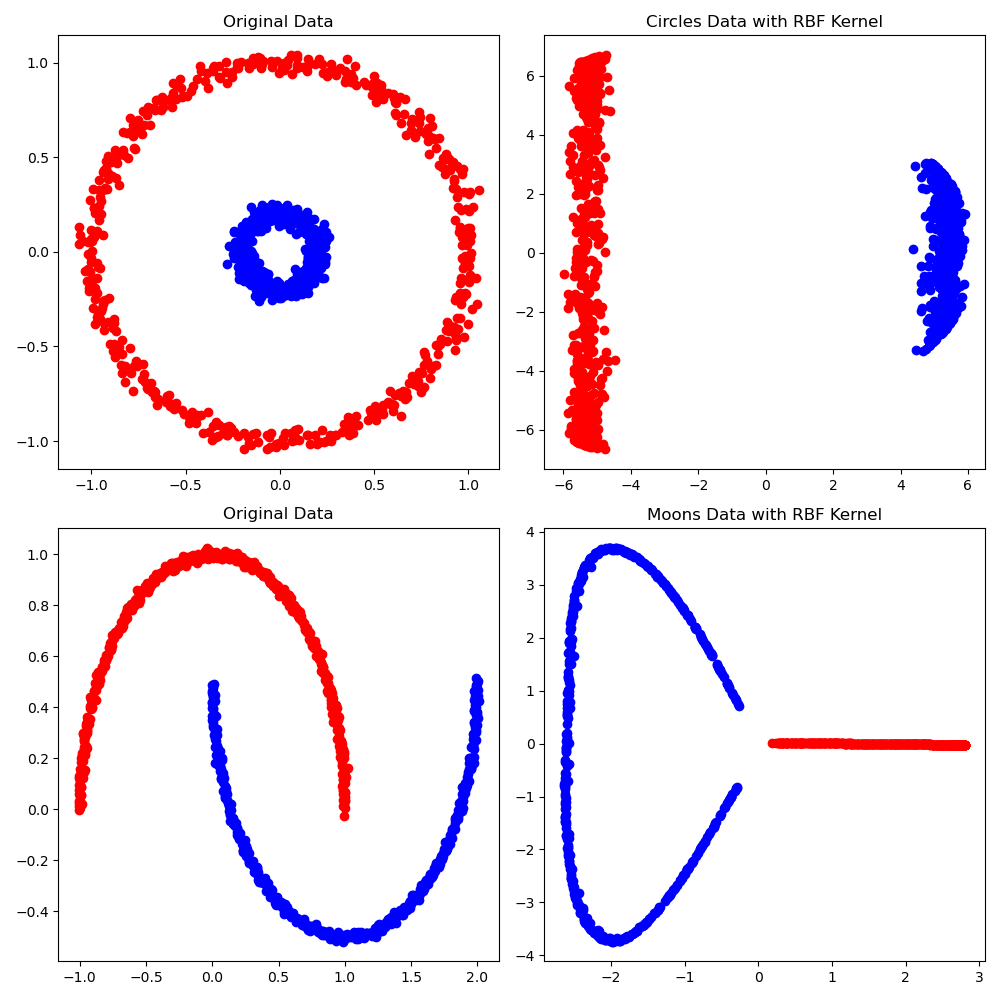
\includegraphics[width=1\textwidth]{../resources/methods/kpca.png}
        \end{center}
    \end{columns}
\end{frame}

\begin{frame}[allowframebreaks]{Principal Component Analysis (Анализ главных компонент, PCA)}
    \textbf{Основная идея:} Нахождение ортогональных направлений (главных компонент), вдоль которых дисперсия максимальна.

    \textbf{Ключевой момент:} Собственные векторы матрицы ковариации данных будут являться главными компонентами.

    \begin{center}
        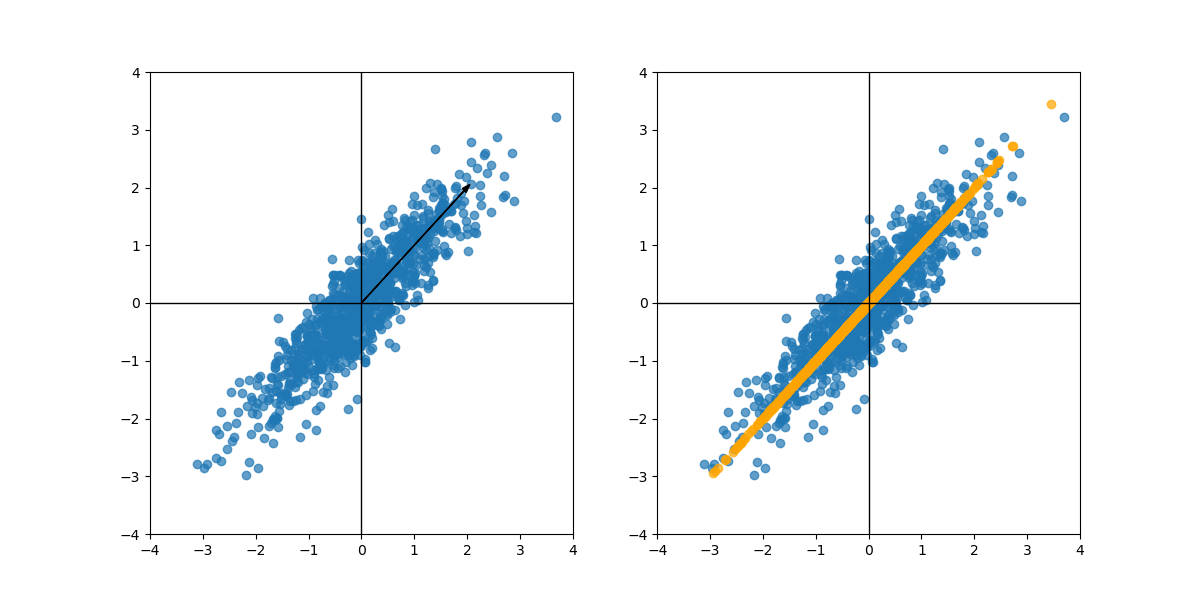
\includegraphics[width=.65\textwidth]{../resources/methods/pca.png}
    \end{center}

    \begin{center}
        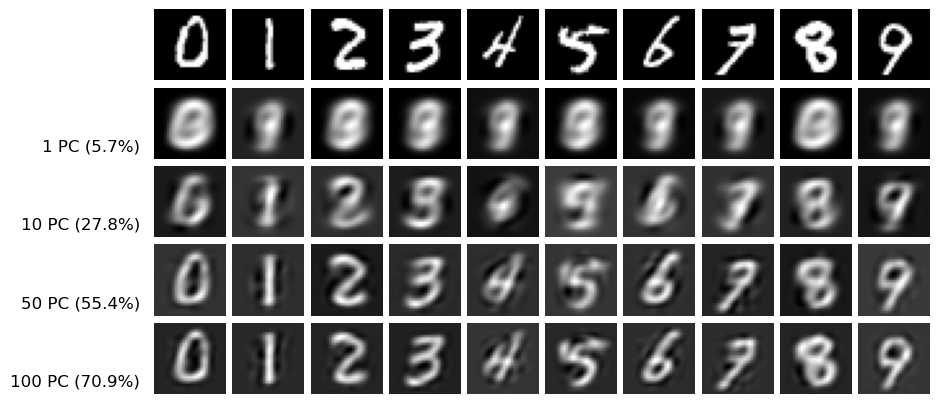
\includegraphics[width=1\textwidth]{../resources/pca/mnist_compression_demo.png}
    \end{center}

\end{frame}

\begin{frame}[allowframebreaks]{Kernel PCA (Ядерный PCA, KPCA)}
    \begin{columns}
        \column{0.5\textwidth}
        \textbf{Основная идея:} Применить PCA в пространстве более высокой размерности.

        \textbf{Ключевой момент:} Использование \textit{ядерного трюка} для избежания прямого преобразования данных в пространство высокой размерности.

        \column{0.55\textwidth}
        \begin{center}
            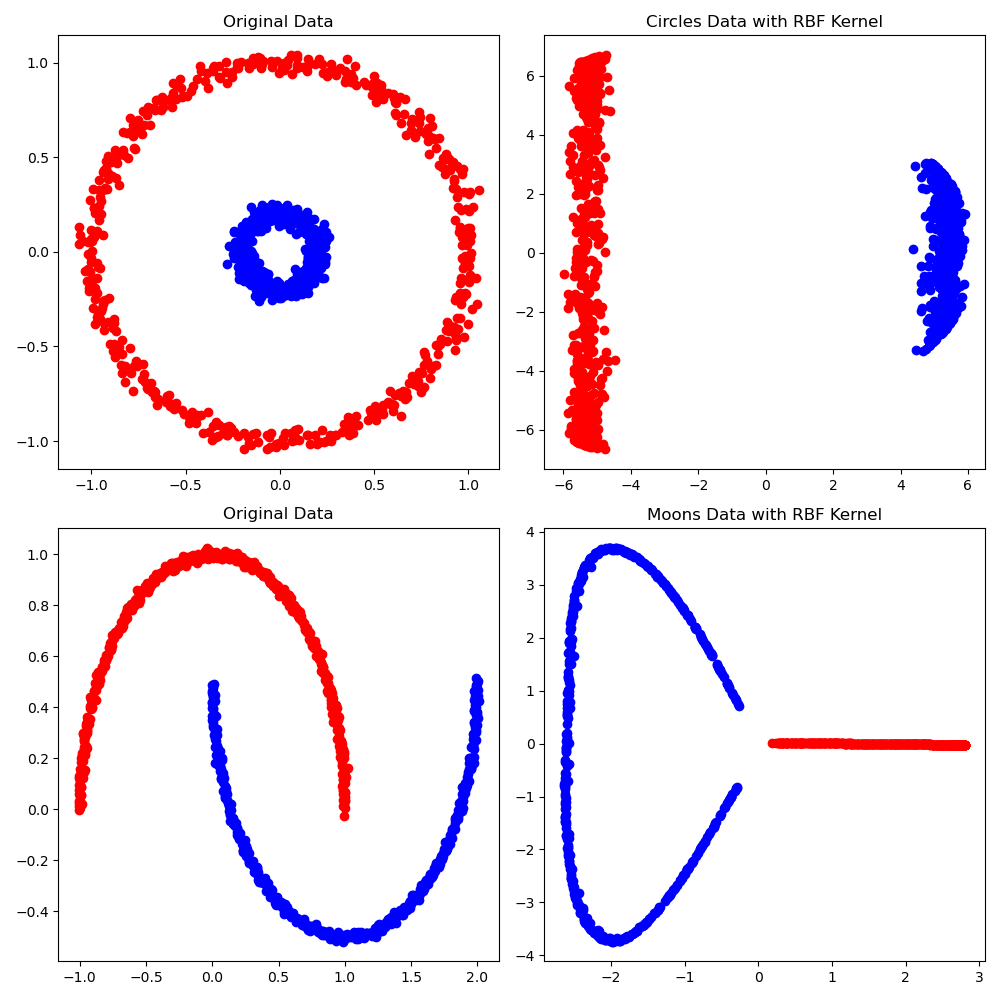
\includegraphics[width=1\textwidth]{../resources/methods/kpca.png}
        \end{center}
    \end{columns}

    \begin{columns}
        \column{0.55\textwidth}
        \begin{center}
            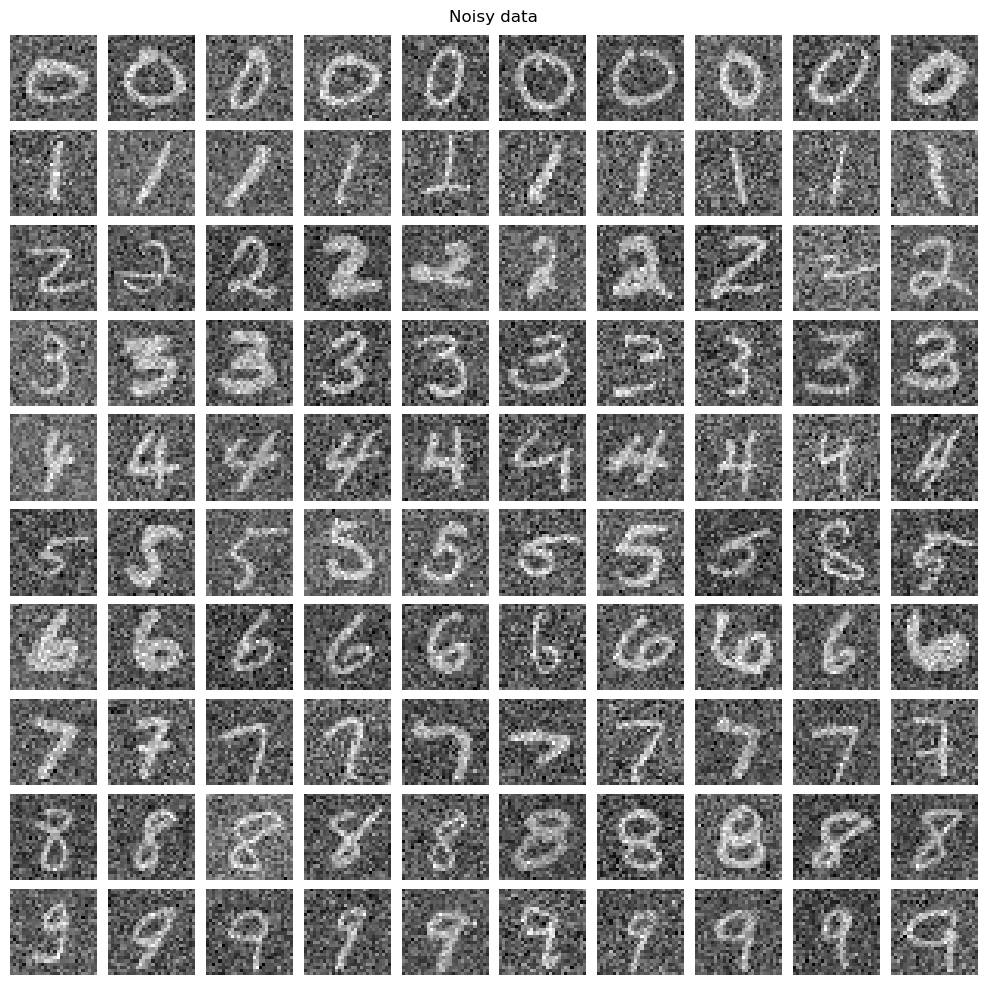
\includegraphics[width=1\textwidth]{../resources/kpca/mnist_noisy.png}
        \end{center}

        \column{0.55\textwidth}
        \begin{center}
            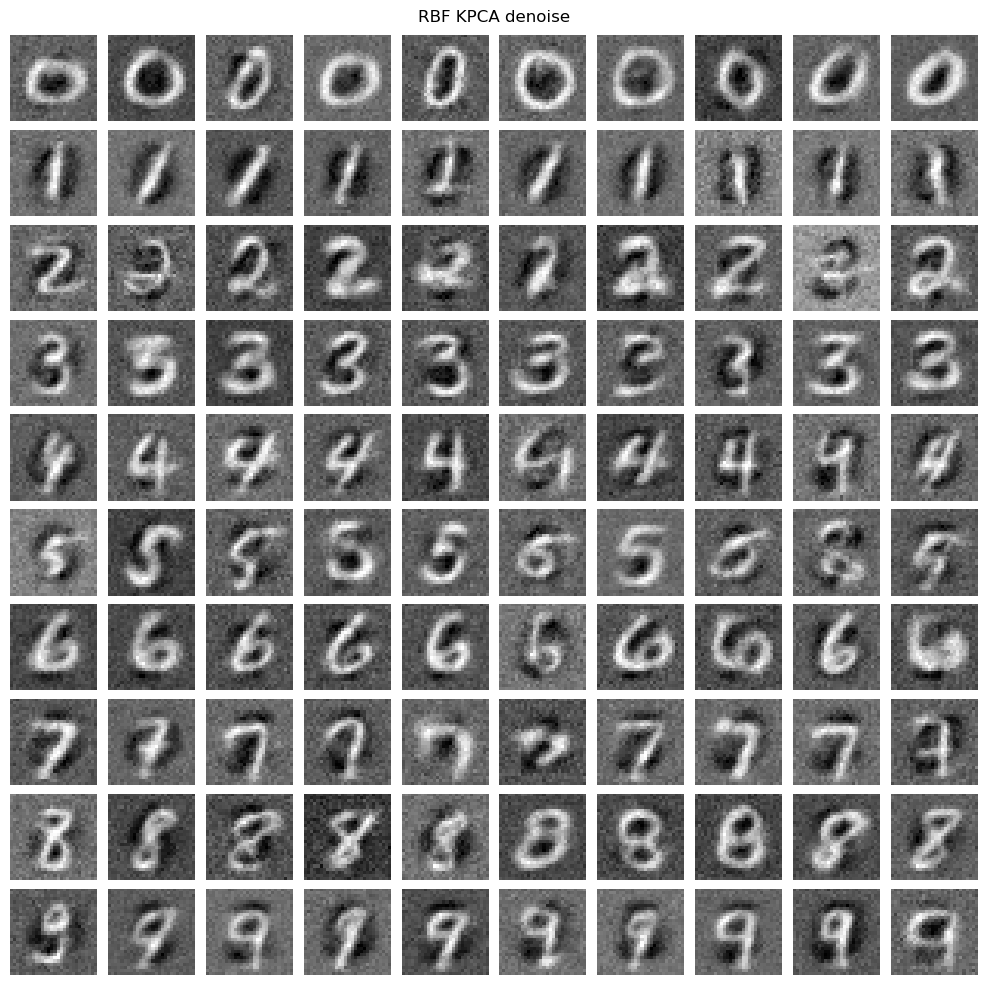
\includegraphics[width=1\textwidth]{../resources/kpca/mnist_denoise_kpca.png}
        \end{center}
    \end{columns}
\end{frame}

\begin{frame}[allowframebreaks]{AutoEncoders (AEs)}
    \textbf{Основная идея:} Нахождение компактных нелинейных представлений данных.

    \textbf{Ключевой момент:} Использование нейронных сетей, обучающихся восстанавливать входные данные, для построения нелинейных преобразований.

    \begin{columns}
        \column{0.55\textwidth}

        \textbf{Архитектура:}
        \begin{itemize}
            \item Кодировщик (encoder): преобразует входные данные в компактное представление.
            \item Декодировщик (decoder): восстанавливает данные из сжатого представления.
        \end{itemize}

        \column{0.45\textwidth}

        \begin{center}
            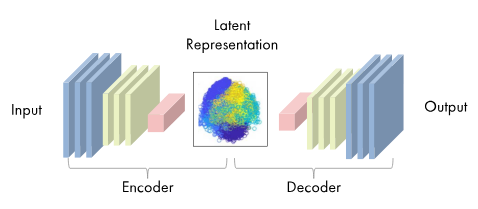
\includegraphics[width=1\textwidth]{../resources/methods/autoencoder.png}
        \end{center}
    \end{columns}

    \begin{columns}
        \column{0.55\textwidth}
        \begin{center}
            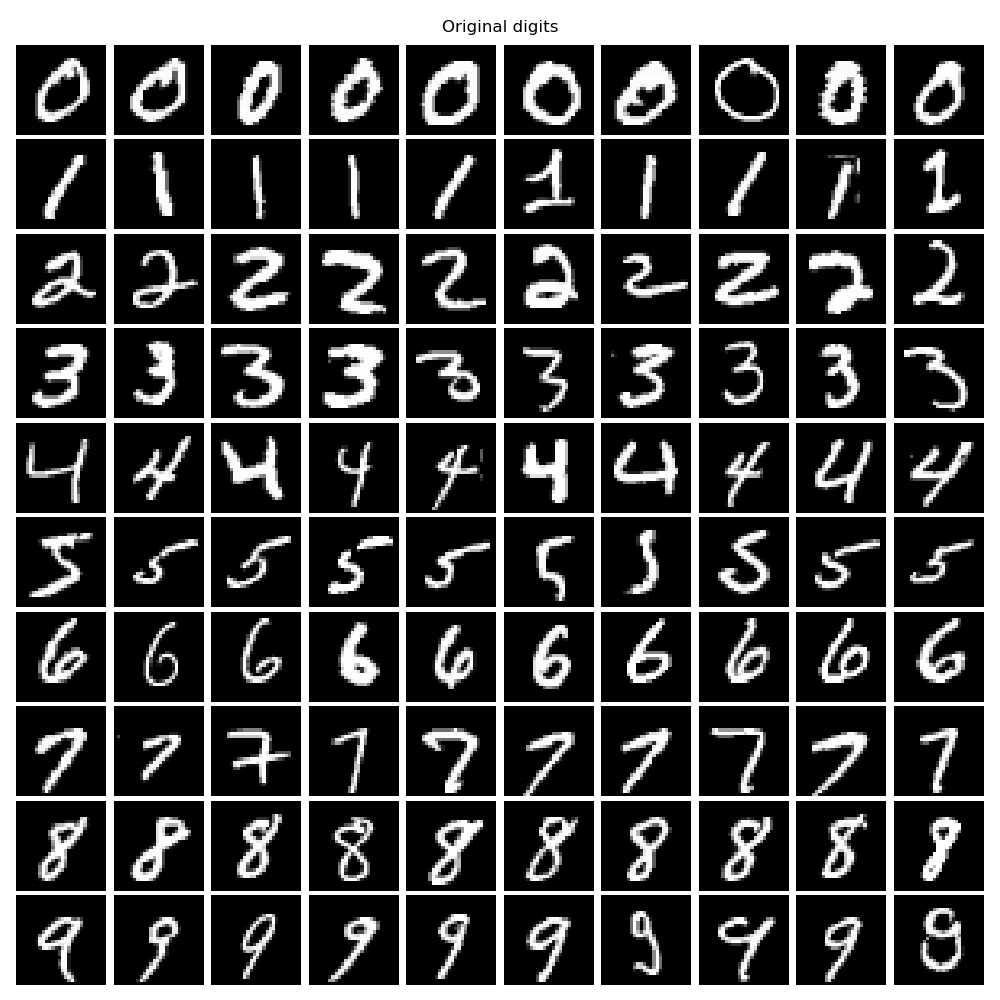
\includegraphics[width=1\textwidth]{../resources/ae/mnist_original_digits.png}
        \end{center}

        \column{0.55\textwidth}
        \begin{center}
            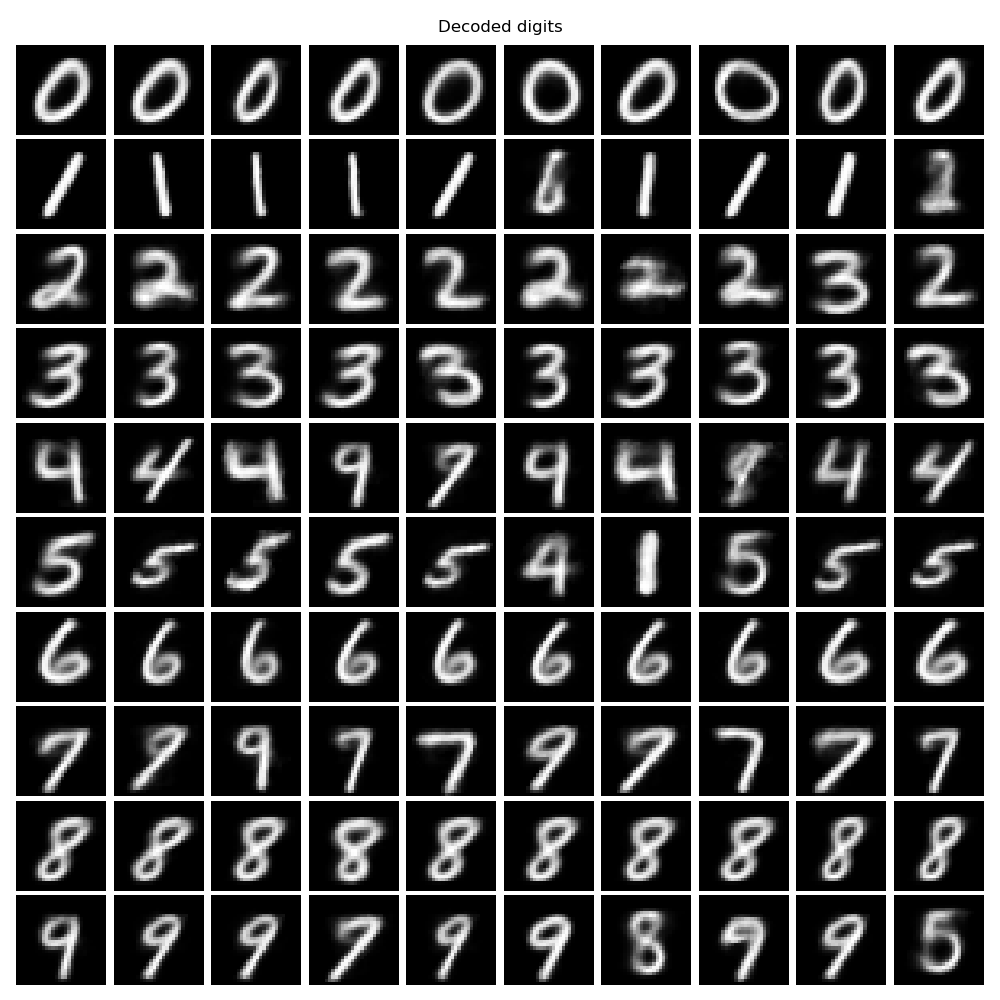
\includegraphics[width=1\textwidth]{../resources/ae/mnist_decoded_digits.png}
        \end{center}
    \end{columns}

    \begin{center}
        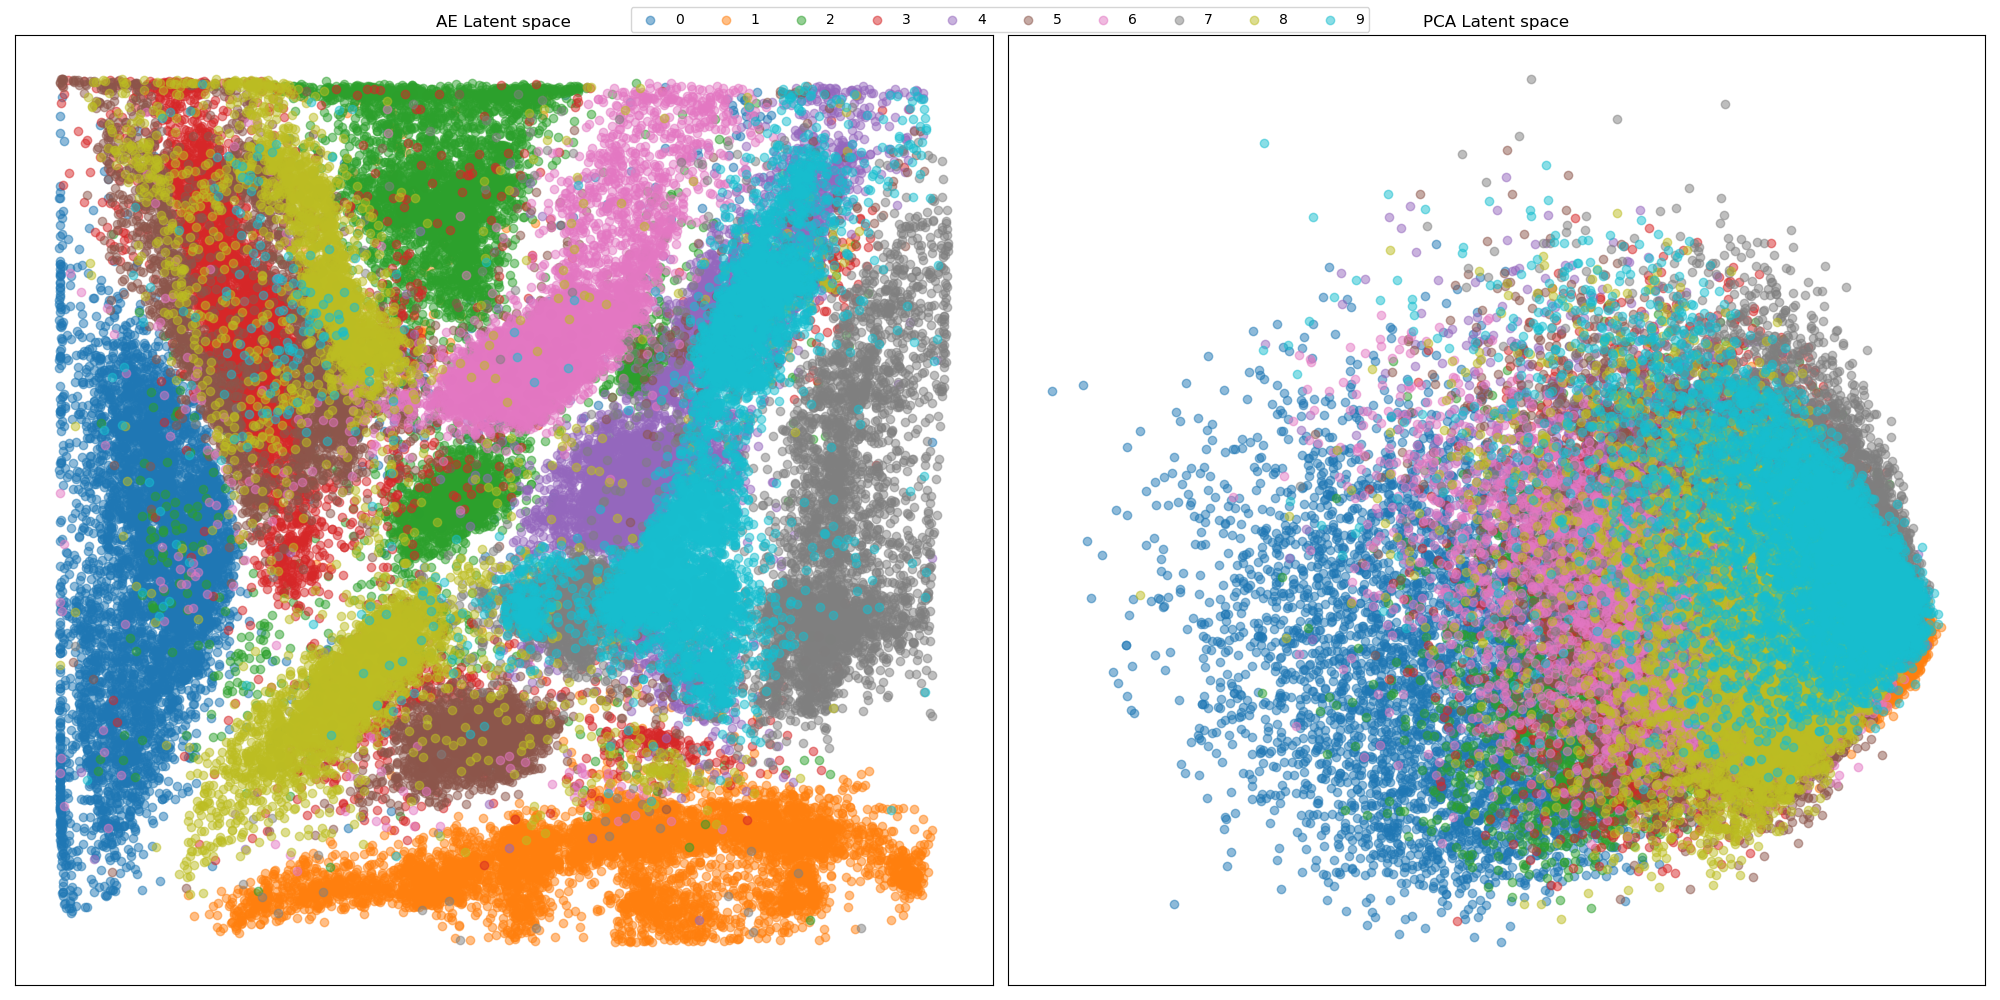
\includegraphics[width=1\textwidth]{../resources/ae/mnist_latent_spaces.png}
    \end{center}

    \begin{center}
        \begin{minipage}{0.32\textwidth}
            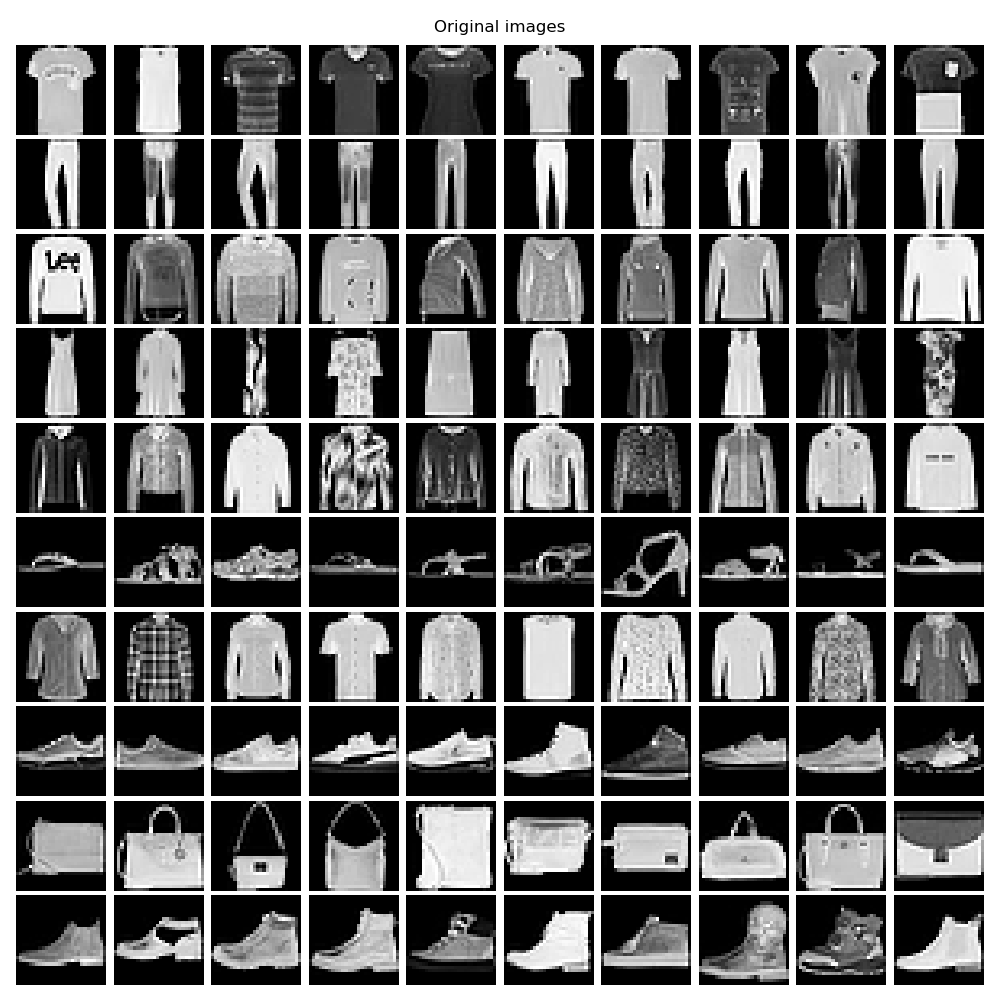
\includegraphics[width=\textwidth]{../resources/ae/fashion_mnist.png}
        \end{minipage}
        \begin{minipage}{0.32\textwidth}
            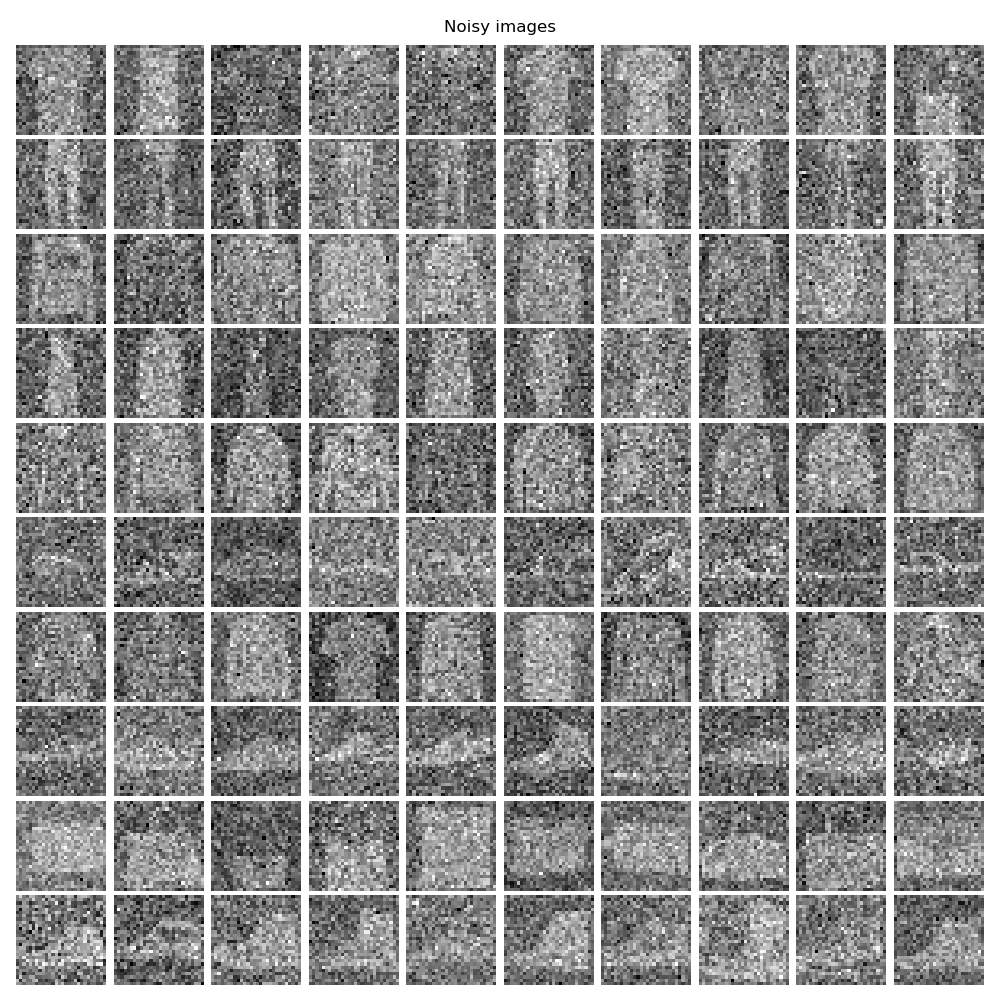
\includegraphics[width=\textwidth]{../resources/ae/fashion_mnist_noisy.png}
        \end{minipage}
        \begin{minipage}{0.32\textwidth}
            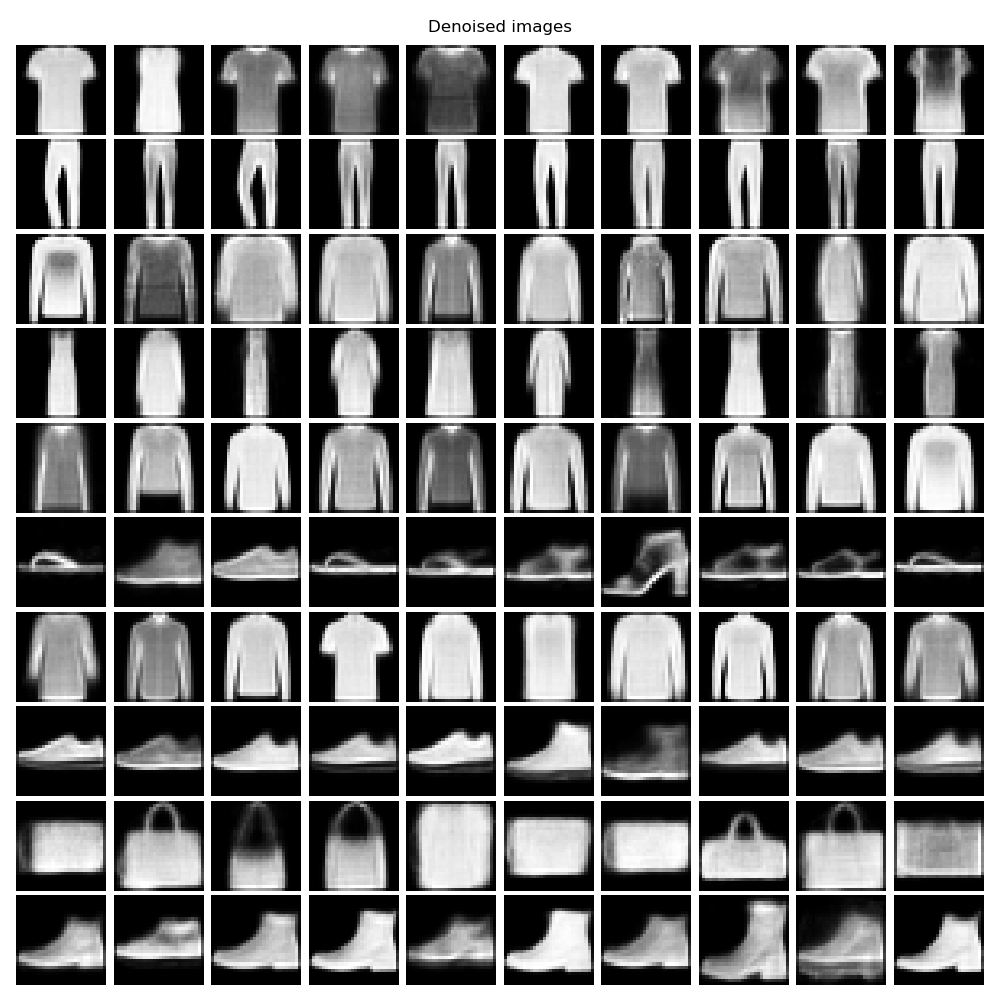
\includegraphics[width=\textwidth]{../resources/ae/fashion_mnist_denoised.png}
        \end{minipage}
    \end{center}
\end{frame}

\begin{frame}[allowframebreaks]{Variational AutoEncoders (VAEs)}
    \textbf{Основная идея: } Представление скрытого пространства в виде вероятностного распределения, что позволит генерировать новые данные.

    \begin{figure}
        \centering
        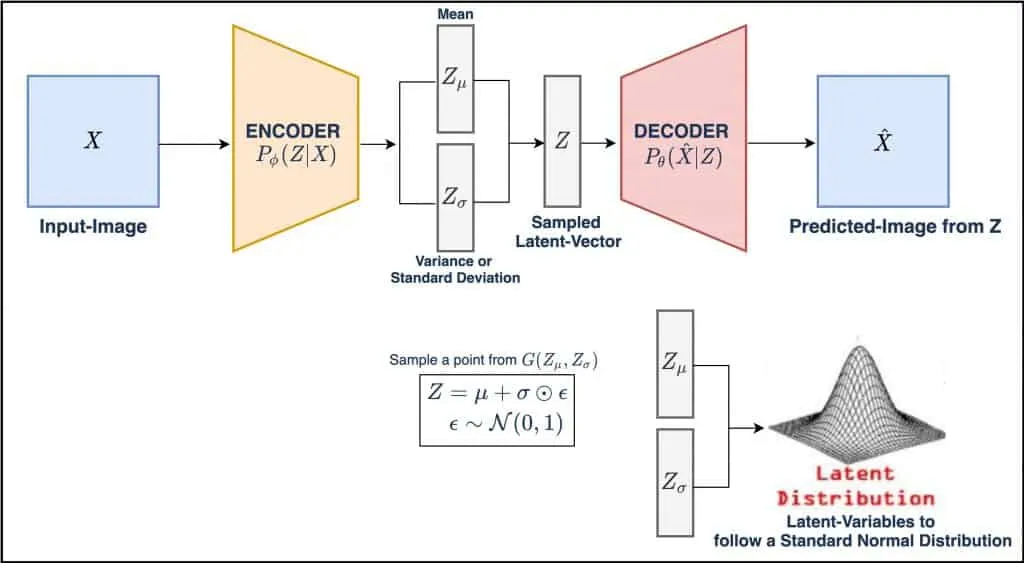
\includegraphics[width=0.6\textwidth]{../resources/methods/vae.png}
    \end{figure}

    \begin{columns}
        \column{0.55\textwidth}
        \begin{center}
            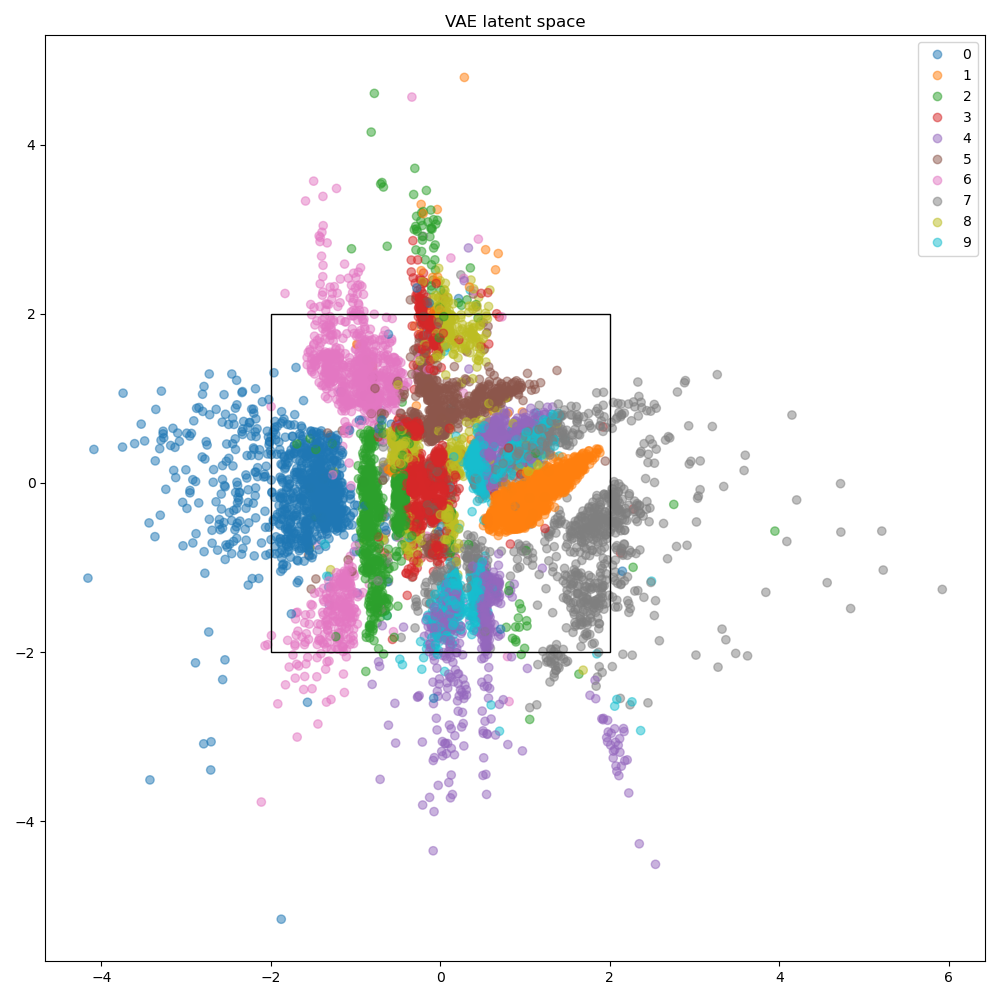
\includegraphics[width=1\textwidth]{../resources/vae/vae_latent_space_scatter.png}
        \end{center}

        \column{0.55\textwidth}
        \begin{center}
            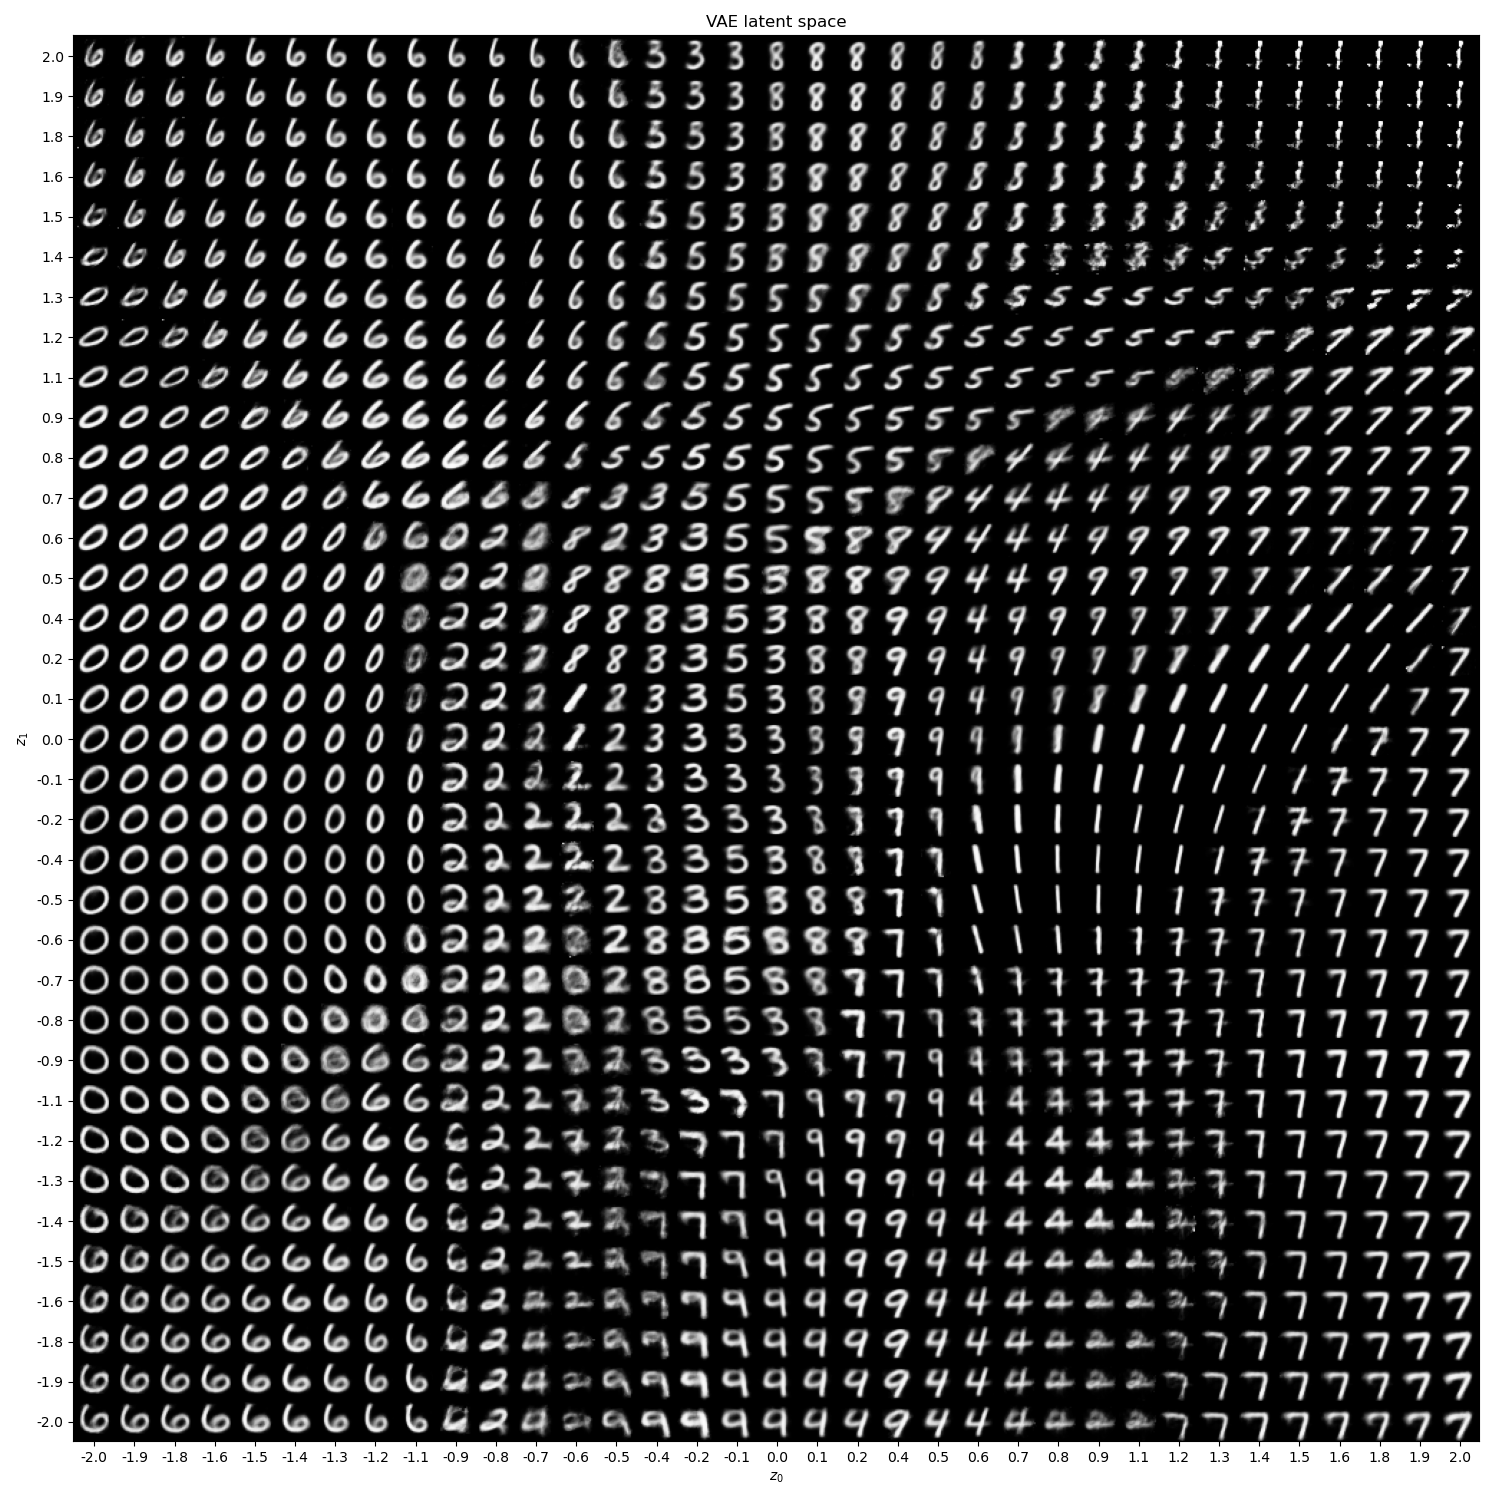
\includegraphics[width=1\textwidth]{../resources/vae/vae_latent_space_sample.png}
        \end{center}
    \end{columns}    
\end{frame}

\section{Principal Component Analysis (\textit{PCA})}

\begin{frame}[allowframebreaks]{Постановка задачи}
    Дан неразмеченный датасет $X = \{\boldsymbol{x}_i\}_{i=1}^N$, где $\boldsymbol{x}_i \in \mathbb{R}^D$.
    Предполагаем центрированность данных: $\mathbb{E}[\boldsymbol{x}_i] = 0$.

    Матрица ковариации данных:
    \begin{equation*}
        \boldsymbol{\Sigma} = \frac{1}{N}\sum_{i=1}^N\boldsymbol{x}_i\boldsymbol{x}_i^T.
    \end{equation*}

    Переход в новое пространство меньшей размерности (сжатие):
    \begin{equation*}
        \boldsymbol{z}_i = \mathbf{B}^T\boldsymbol{x}_i \in \mathbb{R}^M, \quad M<D,
    \end{equation*}

    \framebreak

    Базис $\mathbf{B} = [\boldsymbol{b}_1, \ldots, \boldsymbol{b}_M] \in \mathbb{R}^{D \times M}$ удовлетворяет:
    \begin{equation*}
        \boldsymbol{b}_i^T \boldsymbol{b}_j = \delta_{ij} = \begin{cases}
            0, & i\neq j, \\
            1, & i=j.
        \end{cases}
    \end{equation*}

    Восстановление данных:
    \begin{equation*}
        \tilde{\boldsymbol{x}}_i = \mathbf{B}\boldsymbol{z}_i.
    \end{equation*}
\end{frame}

\begin{frame}{Пример: 2D \(\to\) 1D}
    Исходный вектор: $\boldsymbol{x}_i \in \mathbb{R}^2$, $\boldsymbol{x}_i = \begin{bmatrix} 5 \\ \frac{1}{100} \end{bmatrix}$.
    Выбираем базис $\mathbf{B} = \begin{bmatrix} 1 \\ 0 \end{bmatrix}$.

    \begin{columns}
        \column{0.5\textwidth}
        \textbf{Шаги:}
        \begin{itemize}
            \item Координаты в новом базисе: $\boldsymbol{z}_i = \mathbf{B}^T\boldsymbol{x}_i = 5.$
            \item Восстановленный вектор: $\tilde{\boldsymbol{x}}_i = \mathbf{B}\boldsymbol{z}_i = \begin{bmatrix} 5 \\ 0 \end{bmatrix}.$
        \end{itemize}

        \column{0.55\textwidth}
        \begin{center}
            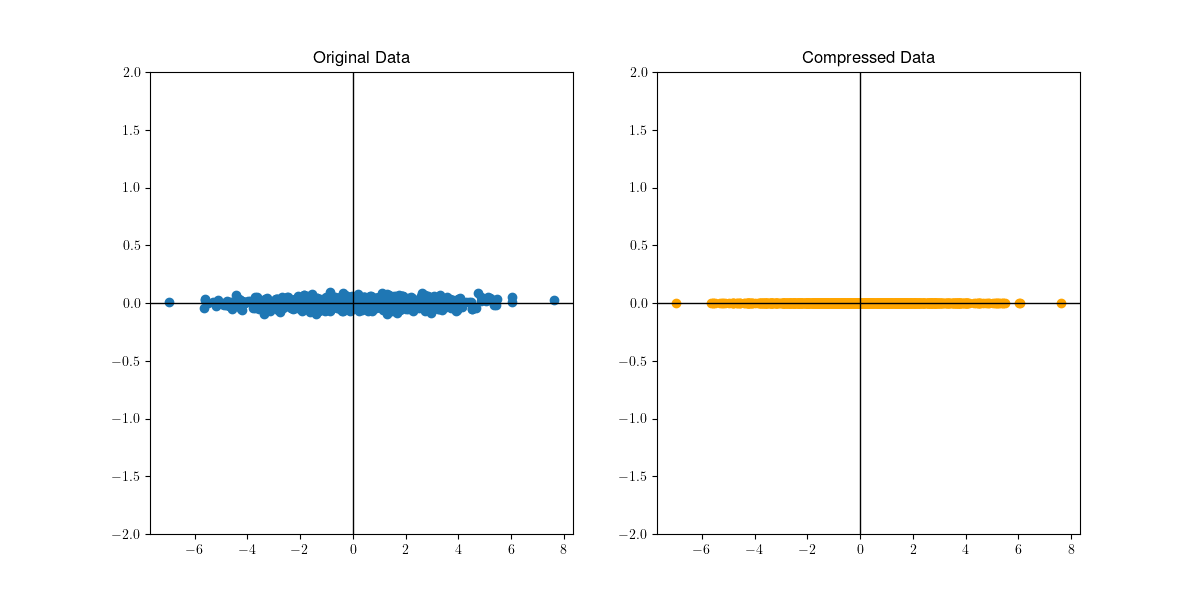
\includegraphics[width=1\textwidth]{../resources/pca/simple_example_both.png}
        \end{center}
    \end{columns}
\end{frame}

\begin{frame}[allowframebreaks]{Нахождение направления максимальной дисперсии}
    \textbf{Цель:} Найти направление $\boldsymbol{b}_1$, вдоль которого дисперсия данных максимальна.

    Дисперсия вдоль первой координаты в новом пространстве:
    \begin{align*}
        V_1 := \mathbb{D}[z_1] & = \frac{1}{N}\sum_{i=1}^Nz_{1i}^2 = \frac{1}{N}\sum_{i=1}^N(\boldsymbol{b}_1^T\boldsymbol{x}_i)^2  = \frac{1}{N}\sum_{i=1}^N(\boldsymbol{b}_1^Tx_ix_i^T\boldsymbol{b}_1) \\
                               & = \boldsymbol{b}_1^T\left(\frac{1}{N}\sum_{i=1}^Nx_ix_i^T\right)\boldsymbol{b}_1 = \boldsymbol{b}_1^T\boldsymbol{\Sigma}\boldsymbol{b}_1.
    \end{align*}

    \framebreak

    Задача условной оптимизации:
    $$
        \max_{\boldsymbol{b}_1} \boldsymbol{b}_1^T \boldsymbol{\Sigma} \boldsymbol{b}_1, \quad\text{s.t.} \: \boldsymbol{b}_1^T \boldsymbol{b}_1 = 1.
    $$

    Функция Лагранжа: \(\mathcal{L}(\boldsymbol{b}_1, \lambda) = \boldsymbol{b}_1^T \boldsymbol{\Sigma} \boldsymbol{b}_1 - \lambda(\boldsymbol{b}_1^T \boldsymbol{b}_1 - 1)\).

    Частные производные по $\boldsymbol{b}_1$ и $\lambda$:

    \begin{align*}
        \frac{\partial\mathcal{L}}{\partial\boldsymbol{b}_1} & = 2\boldsymbol{\Sigma}\boldsymbol{b}_1 - 2\lambda_1\boldsymbol{b}_1 = 0, \\
        \frac{\partial\mathcal{L}}{\partial\lambda_1}        & = -\boldsymbol{b}_1^T\boldsymbol{b}_1 + 1 = 0.
    \end{align*}
\end{frame}

\begin{frame}{Собственные векторы и значения}
    \textbf{Получаем:}
    \begin{align*}
        \boldsymbol{\Sigma} \boldsymbol{b}_1 & = \lambda_1 \boldsymbol{b}_1, \\
        V_1                                  & = \lambda_1.
    \end{align*}

    Теперь можем переписать дисперсию $V_1$ как:

    $$
        V_1 = \boldsymbol{b}_1^T\boldsymbol{\Sigma}\boldsymbol{b}_1 = \lambda_1\boldsymbol{b}_1^T\boldsymbol{b}_1 = \lambda_1.
    $$

    \textbf{Интерпретация:}
    \begin{itemize}
        \item $\boldsymbol{b}_1$: первое направление главной компоненты.
        \item $\lambda_1$: дисперсия вдоль направления $\boldsymbol{b}_1$.
    \end{itemize}
\end{frame}

\begin{frame}[allowframebreaks]{Остальные компоненты}
    \textbf{Для $m$-й компоненты:}
    \begin{align*}
         & \max_{\boldsymbol{b}_m} \boldsymbol{b}_m^T \boldsymbol{\Sigma} \boldsymbol{b}_m,                                    \\
         & \text{s.t. } \boldsymbol{b}_m^T \boldsymbol{b}_m = 1, \quad \boldsymbol{b}_m^T \boldsymbol{b}_i = 0, \forall i < m.
    \end{align*}

    Функция Лагранжа: \(
    \mathcal{L}(\boldsymbol{b}_m, \lambda_m, \boldsymbol{\mu}) = \boldsymbol{b}_m^T\boldsymbol{\Sigma}\boldsymbol{b}_m - \lambda_m(\boldsymbol{b}_m^T\boldsymbol{b}_m - 1) - \sum_{i=1}^{m-1}\mu_i\boldsymbol{b}_m^T\boldsymbol{b}_i.
    \)

    \begin{align*}
        \frac{\partial\mathcal{L}}{\partial\boldsymbol{b}_m} & = 2\boldsymbol{\Sigma}\boldsymbol{b}_m - 2\lambda_m\boldsymbol{b}_m - \sum_{i=1}^{m-1}\mu_i\boldsymbol{b}_i = 0, \\
        \frac{\partial\mathcal{L}}{\partial\lambda_m}        & = -\boldsymbol{b}_m^T\boldsymbol{b}_m + 1 = 0,\quad
        \frac{\partial\mathcal{L}}{\partial\mu_i} = -\boldsymbol{b}_m^T\boldsymbol{b}_i = 0,\:\forall i<m.
    \end{align*}

    Домножим первое уравнение на $\boldsymbol{b}_j^T,\:j<m$ слева:

    $$
        2\boldsymbol{b}_j^T\boldsymbol{\Sigma}\boldsymbol{b}_m - 2\lambda_m\boldsymbol{b}_j^T\boldsymbol{b}_m - \sum_{i=1}^{m-1}\mu_i\boldsymbol{b}_j^T\boldsymbol{b}_i = 0,
    $$

    поскольку $\boldsymbol{b}_j^T\boldsymbol{b}_i = \delta_{ji}$:

    $$
        2\boldsymbol{b}_j^T\boldsymbol{\Sigma}\boldsymbol{b}_m - \mu_j = 0.
    $$

    $\boldsymbol{\Sigma}$ симметрична, поэтому $\boldsymbol{b}_j^T\boldsymbol{\Sigma}\boldsymbol{b}_m = \left\langle (\boldsymbol{b}_j^T\boldsymbol{\Sigma})^T, \boldsymbol{b}_m \right\rangle = \left\langle \boldsymbol{\Sigma}\boldsymbol{b}_j, \boldsymbol{b}_m \right\rangle = \left\langle \lambda_j\boldsymbol{b}_j, \boldsymbol{b}_m \right\rangle = \lambda_j \left\langle \boldsymbol{b}_j, \boldsymbol{b}_m \right\rangle = 0$.

    Тогда $\mu_j = 0.$ и, аналогично, $\forall j<m \:\: \mu_j=0$

    \framebreak

    Таким образом:

    $$
        \boldsymbol{\Sigma}\boldsymbol{b}_m = \lambda_m\boldsymbol{b}_m,
    $$

    Вновь, $\boldsymbol{b}_m$ - собственный вектор матрицы ковариации $\boldsymbol{\Sigma}$, а $\lambda_m$ - собственное значение.

    \textbf{Общая дисперсия:} $\sum_{i=1}^N\lambda_i$. \\
    \textbf{Объясненная дисперсия} первых $m$ главных компонент: $\sum_{i=1}^m\lambda_i$. \\
    \textbf{Доля объясненной дисперсии:} $\frac{\sum_{i=1}^m\lambda_i}{\sum_{i=1}^N\lambda_i}$.
\end{frame}

\begin{frame}{Практические аспекты реализации}
    \textbf{Формулы:}
    \begin{align*}
        \boldsymbol{Z}         & = \mathbf{B}^T \boldsymbol{X},                \\
        \tilde{\boldsymbol{X}} & = \mathbf{B} \boldsymbol{Z},                  \\
        \boldsymbol{\Sigma}    & = \frac{1}{N}\boldsymbol{X} \boldsymbol{X}^T.
    \end{align*}

    \textbf{Примечание:} строки \(\boldsymbol{X}\) — признаки, столбцы — объекты.
\end{frame}

\begin{frame}{Практика}
    \begin{figure}
        \centering
        
\includegraphics[width=.3\textwidth]{../resources/overall/Jupyter_logo.png}
    \end{figure}
\end{frame}

\section{Kernel PCA (\textit{KPCA})}

\begin{frame}[allowframebreaks]{Постановка задачи}
    Дан центрированный неразмеченный датасет $X = \{\boldsymbol{x}_i\}_{i=1}^N$, $\boldsymbol{x}_i \in \mathbb{R}^D$.

    Задано:
    \begin{itemize}
        \item Преобразование $\phi: \mathbb{R}^D \to \mathbb{H}$, где $\mathbb{H}$ — гильбертово пространство.
        \item Функция (ядро) $k: \mathbb{R}^D \times \mathbb{R}^D \to \mathbb{R}:\quad k(\boldsymbol{x}, \boldsymbol{y}) = \langle\phi(\boldsymbol{x}), \phi(\boldsymbol{y})\rangle_{\mathbb{H}}.$
    \end{itemize}

    \textbf{Цель:} Найти линейное подпространство в $\mathbb{H}$ размерности $P$, минимизирующее расстояние между $x_i$ и их проекцией.

    \framebreak

    \textbf{Свойства ядерных функций:}
    \begin{itemize}
        \item \textbf{Утверждение:} по произвольной функции $\phi$ можно построить ядро $k$ - положительно определенная функция.
        \item \textbf{Теорема Moore-Aronszajn:} По положительно определённому ядру $k$ можно построить $\phi$ и пространство $\mathbb{H}$.
        \item Матрица Грама $\mathbf{K} \in \mathbb{R}^{N \times N}$:
              \begin{equation*}
                  K_{ij} = k(\boldsymbol{x}_i, \boldsymbol{x}_j).
              \end{equation*}
    \end{itemize}

    \textbf{Пространство:} Пусть $\mathbb{H} = \mathbb{R}^H$, где $H \gg D$ (для конечномерного случая).
\end{frame}

\begin{frame}{Наивный подход}
    \textbf{Шаги:}
    \begin{enumerate}
        \item Вычислить $\{\phi(\boldsymbol{x}_i)\}_{i=1}^N$.
        \item Применить PCA к $\{\phi(\boldsymbol{x}_i)\}_{i=1}^N$.
    \end{enumerate}

    \textbf{Проблемы:}
    \begin{itemize}
        \item Вычисление $\phi(\boldsymbol{x}_i)$ дорого.
        \item $\phi$ может быть неизвестным.
        \item Ковариационная матрица размера $H \times H$, где $H \gg D$.
    \end{itemize}
\end{frame}

\begin{frame}[allowframebreaks]{Kernel Trick}
    \textbf{Подход:}
    Составим из $\phi(\boldsymbol{x}_i)$ матрицу $\boldsymbol{\Phi}$ ($N \times H$). Матрица ковариации:
    \begin{equation*}
        \boldsymbol{\Sigma} = \frac{1}{N}\sum_{i=1}^N\phi(\boldsymbol{x}_i)\phi(\boldsymbol{x}_i)^T = \frac{1}{N}\boldsymbol{\Phi}^T\boldsymbol{\Phi}.
    \end{equation*}

    Главные компоненты $\mathbf{\omega}_p \in \mathbb{H}$:
    \begin{equation*}
        \boldsymbol{\Sigma}\mathbf{\omega}_p = \lambda_p\mathbf{\omega}_p \quad \text{для } p = 1, 2, \ldots, P.
    \end{equation*}

    \framebreak

    Подставим $\boldsymbol{\Sigma}$:

    \begin{align*}
         & \frac{1}{N}\sum_{i=1}^N\phi(\boldsymbol{x}_i)\phi(\boldsymbol{x}_i)^T\mathbf{\omega}_p =  \frac{1}{N}\sum_{i=1}^N\phi(\boldsymbol{x}_i)\langle\phi(\boldsymbol{x}_i), \mathbf{\omega}_p\rangle_{\mathbb{H}} = \lambda_p\mathbf{\omega}_p.
    \end{align*}

    \textbf{Представление компонент:}
    \begin{equation*}
        \mathbf{\omega}_p = \sum_{j=1}^N \alpha_{p,j}\phi(\boldsymbol{x}_j), \quad \alpha_{p,j} = \langle\phi(\boldsymbol{x}_j), \mathbf{\omega}_p\rangle_{\mathbb{H}}.
    \end{equation*}

    \framebreak

    Подставим это в уравнение для $\mathbf{\omega}_p$:

    \begin{align*}
         & \frac{1}{N}\sum_{i=1}^N\phi(\boldsymbol{x}_i)\langle\phi(\boldsymbol{x}_i), \sum_{j=1}^N\alpha_{p,j}\phi(\boldsymbol{x}_j)\rangle_{\mathbb{H}} = \lambda_p\sum_{i=1}^N\alpha_{p,i}\phi(\boldsymbol{x}_i), \\
         & \frac{1}{N}\sum_{i=1}^N\phi(\boldsymbol{x}_i)\phi(\boldsymbol{x}_i)^T\sum_{j=1}^N\phi(\boldsymbol{x}_j)\alpha_{p,j} = \lambda_p\sum_{j=1}^N\alpha_{p,j}\phi(\boldsymbol{x}_j),                            \\
         & \frac{1}{N}\boldsymbol{\Phi}^T\boldsymbol{\Phi}\boldsymbol{\Phi}^T\boldsymbol{\alpha}_p = \lambda_p\boldsymbol{\Phi}^T\boldsymbol{\alpha}_p,                                                              \\
         & \boldsymbol{\Phi}^T(\boldsymbol{\Phi}\boldsymbol{\Phi}^T\boldsymbol{\alpha}_p - N\lambda_p\boldsymbol{\alpha}_p) = 0                                                                                      \\
         & \mathbf{K}\boldsymbol{\alpha}_p = N\lambda_p\boldsymbol{\alpha}_p, \hspace{1cm} \mathbf{K} = \boldsymbol{\Phi}\boldsymbol{\Phi}^T, \hspace{1cm} K_{ij} = k(\boldsymbol{x}_i, \boldsymbol{x}_j).
    \end{align*}
\end{frame}

\begin{frame}{Проекции на главные компоненты}
    Проекции на главные компоненты вычисляются \textbf{даже без знания $\phi$}:

    \begin{align*}
        \boldsymbol{z}_{ij} & = \langle\phi(\boldsymbol{x}_i), \mathbf{\omega}_j\rangle_{\mathbb{H}} = \boldsymbol{\omega}_j^T\phi(\boldsymbol{x}_i) = \sum_{k=1}^N\alpha_{j,k}\phi(\boldsymbol{x}_k)^T\phi(\boldsymbol{x}_i) \\
                            & = \sum_{k=1}^N\alpha_{j,k}k(\boldsymbol{x}_k, \boldsymbol{x}_i) = \sum_{k=1}^N\alpha_{j,k}\mathbf{K}_{ki} = \sum_{k=1}^N\alpha_{j,k}\mathbf{K}_{ik} = \mathbf{K}_i\boldsymbol{\alpha}_j. \\ \\
        \mathbf{Z}         & = \mathbf{K}\boldsymbol{\mathbf{\alpha}}.
    \end{align*}

\end{frame}

\begin{frame}[allowframebreaks]{Центрирование образов}
    \textbf{Проблема:}
    Образы $\phi(\boldsymbol{x}_i)$ могут быть нецентрированными, даже если $\boldsymbol{x}_i$ центрированы.

    \textbf{Коррекция:}
    \begin{equation*}
        \tilde{\phi}(\boldsymbol{x}) = \phi(\boldsymbol{x}) - \frac{1}{N}\sum_{i=1}^N\phi(\boldsymbol{x}_i).
    \end{equation*}

    \framebreak

    \textbf{Обновление ядра:}
    \begin{align*}
        \tilde{k}(\boldsymbol{x}, \boldsymbol{y}) & = k(\boldsymbol{x}, \boldsymbol{y}) - \frac{1}{N}\sum_{i=1}^N\left(k(\boldsymbol{x}, \boldsymbol{x}_i) - k(\boldsymbol{x}_i, \boldsymbol{y})\right) \\
                                                  & \quad + \frac{1}{N^2}\sum_{i=1}^N\sum_{j=1}^N k(\boldsymbol{x}_i, \boldsymbol{x}_j).
    \end{align*}

    Центрированная матрица:
    \begin{equation*}
        \tilde{\mathbf{K}} = \left(\mathbf{E} - \frac{1}{N}\mathbf{1}\mathbf{1}^T\right)\mathbf{K}\left(\mathbf{E} - \frac{1}{N}\mathbf{1}\mathbf{1}^T\right),
    \end{equation*}
    где $\mathbf{1}$ — вектор из единиц.
\end{frame}

\begin{frame}{Детали реализации}
    \textbf{Наиболее популярное ядро:} Гауссово (RBF):
    \begin{equation*}
        k(\boldsymbol{x}, \boldsymbol{y}) = \exp\left(-\frac{\|\boldsymbol{x} - \boldsymbol{y}\|^2}{2\sigma^2}\right) = \exp\left(-\gamma\|\boldsymbol{x} - \boldsymbol{y}\|^2\right).
    \end{equation*}

    \textbf{Альтернативные ядра:}
    \begin{itemize}
        \item Полиномиальное: $k(\boldsymbol{x}, \boldsymbol{y}) = (\gamma\boldsymbol{x}^T\boldsymbol{y} + r)^d$.
        \item Сигмоидальное: $k(\boldsymbol{x}, \boldsymbol{y}) = \tanh(\gamma\boldsymbol{x}^T\boldsymbol{y} + r)$.
        \item Линейное: $k(\boldsymbol{x}, \boldsymbol{y}) = \boldsymbol{x}^T\boldsymbol{y}$.
    \end{itemize}
\end{frame}

\begin{frame}{Практика}
    \begin{figure}
        \centering
        
\includegraphics[width=.3\textwidth]{../resources/overall/Jupyter_logo.png}
    \end{figure}
\end{frame}

\section{AutoEncoders (\textit{AEs})}

\begin{frame}{Постановка задачи}
    Дан неразмеченный датасет $X = \{\boldsymbol{x}_i\}_{i=1}^N$, где $\boldsymbol{x}_i \in \mathbb{R}^D$.

    \textbf{Цель:} Найти сжатое представление $\boldsymbol{z}_i \in \mathbb{R}^M$, $M < D$, такое что восстановленные данные $\tilde{\boldsymbol{x}}_i$ близки к исходным $\boldsymbol{x}_i$.

    \textbf{Подход:} Использование нелинейных преобразований, реализованных нейронной сетью.
\end{frame}

\begin{frame}[allowframebreaks]{Архитектура автоэнкодера}
    \textbf{Encoder:} Нелинейное отображение $f_{\boldsymbol{\theta}}: \mathbb{R}^D \to \mathbb{R}^M$:
    \begin{equation*}
        \boldsymbol{z} = f_{\boldsymbol{\theta}}(\boldsymbol{x}),
    \end{equation*}
    где:
    \begin{equation*}
        f_{\boldsymbol{\theta}} = f_L \circ f_{L-1} \circ \ldots \circ f_1, \quad f_i = \sigma_{\text{E}i}(\mathbf{W}_{\text{E}i}\boldsymbol{z}_{i-1} + \boldsymbol{b}_{\text{E}i}).
    \end{equation*}

    \textbf{Decoder:} Восстановление $g_{\boldsymbol{\phi}}: \mathbb{R}^M \to \mathbb{R}^D$:
    \begin{equation*}
        \tilde{\boldsymbol{x}} = g_{\boldsymbol{\phi}}(\boldsymbol{z}),
    \end{equation*}
    где:
    \begin{equation*}
        g_{\boldsymbol{\phi}} = g_L \circ g_{L-1} \circ \ldots \circ g_1, \quad g_i = \sigma_{\text{D}i}(\mathbf{W}_{\text{D}i}\boldsymbol{z}_{i-1} + \boldsymbol{b}_{\text{D}i}).
    \end{equation*}

    \textbf{Полная архитектура:}
    \begin{align*}
        &\boldsymbol{z} = f_{\boldsymbol{\theta}}(\boldsymbol{x}), \\
        &\tilde{\boldsymbol{x}} = g_{\boldsymbol{\phi}}(\boldsymbol{z}).
    \end{align*}

    \begin{figure}
        \centering
        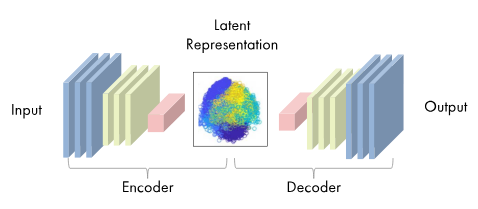
\includegraphics[width=.8\textwidth]{../resources/methods/autoencoder.png}
    \end{figure}
\end{frame}

\begin{frame}{Обучение автоэнкодера}
    \textbf{Функция потерь:} ошибка реконструкции (\textit{reconstruction error}):
    \begin{equation*}
        \mathcal{L}(\boldsymbol{\theta}, \boldsymbol{\phi}) = \frac{1}{N}\sum_{i=1}^N\|\boldsymbol{x}_i - \tilde{\boldsymbol{x}}_i\|^2_2 = \frac{1}{N}\sum_{i=1}^N\|\boldsymbol{x}_i - g_{\boldsymbol{\phi}}(f_{\boldsymbol{\theta}}(\boldsymbol{x}_i))\|^2_2.
    \end{equation*}

    \textbf{Альтернативная функция потерь:} бинарная кросс-энтропия для выхода в $[0, 1]^D$:
    \begin{equation*}
        \mathcal{L}(\boldsymbol{\theta}, \boldsymbol{\phi}) = \frac{1}{N}\sum_{i=1}^N\sum_{j=1}^D\left(x_{ij}\log\tilde{x}_{ij} + (1 - x_{ij})\log(1 - \tilde{x}_{ij})\right).
    \end{equation*}
\end{frame}

\begin{frame}{Аналогия с PCA}
    \textbf{Ошибка реконструкции в PCA:}
    \begin{equation*}
        \mathcal{L}(\boldsymbol{\theta}, \boldsymbol{\phi}) = \frac{1}{N}\sum_{i=1}^N\|\boldsymbol{x}_i - \tilde{\boldsymbol{x}}_i\|^2_2 = \frac{1}{N}\sum_{i=1}^N\|\boldsymbol{x}_i - \mathbf{B}\mathbf{B}^T\boldsymbol{x}_i\|^2_2.
    \end{equation*}

    Если:
    \begin{equation*}
        f_{\boldsymbol{\theta}}(\boldsymbol{x}) = \mathbf{W}_{\text{E}}\boldsymbol{x}, \quad g_{\boldsymbol{\phi}}(\boldsymbol{z}) = \mathbf{W}_{\text{D}}\boldsymbol{z},
    \end{equation*}
    то:
    \begin{equation*}
        \mathbf{W}_{\text{E}} = \mathbf{B}^T, \quad \mathbf{W}_{\text{D}} = \mathbf{B},
    \end{equation*}
    и автоэнкодер эквивалентен PCA.
\end{frame}

\begin{frame}{Практика}
    \begin{figure}
        \centering
        
\includegraphics[width=.3\textwidth]{../resources/overall/Jupyter_logo.png}
    \end{figure}
\end{frame}
\section{Variational AutoEncoders (\textit{VAEs})}

\begin{frame}[allowframebreaks]{Постановка задачи}
    Дан неразмеченный датасет $X = \{\boldsymbol{x}_i\}_{i=1}^N$, где $\boldsymbol{x}_i \in \mathbb{R}^D$.

    \textbf{Цель:}
    \begin{itemize}
        \item Обучить автоэнкодер так, чтобы его скрытое представление $\boldsymbol{z}_i \in \mathbb{R}^M$ было распределено по заданному распределению.
        \item Задать латентное распределение: $p(\boldsymbol{z}) = \mathcal{N}(\boldsymbol{z} \mid \mathbf{0}, \mathbf{E})$.
    \end{itemize}

    \textbf{Построение генеративной модели:}
    \begin{itemize}
        \item Способность генерировать объекты $p(\boldsymbol{z})$, близкие к объектам обучающей выборки $X$.
    \end{itemize}

    \begin{figure}
        \centering
        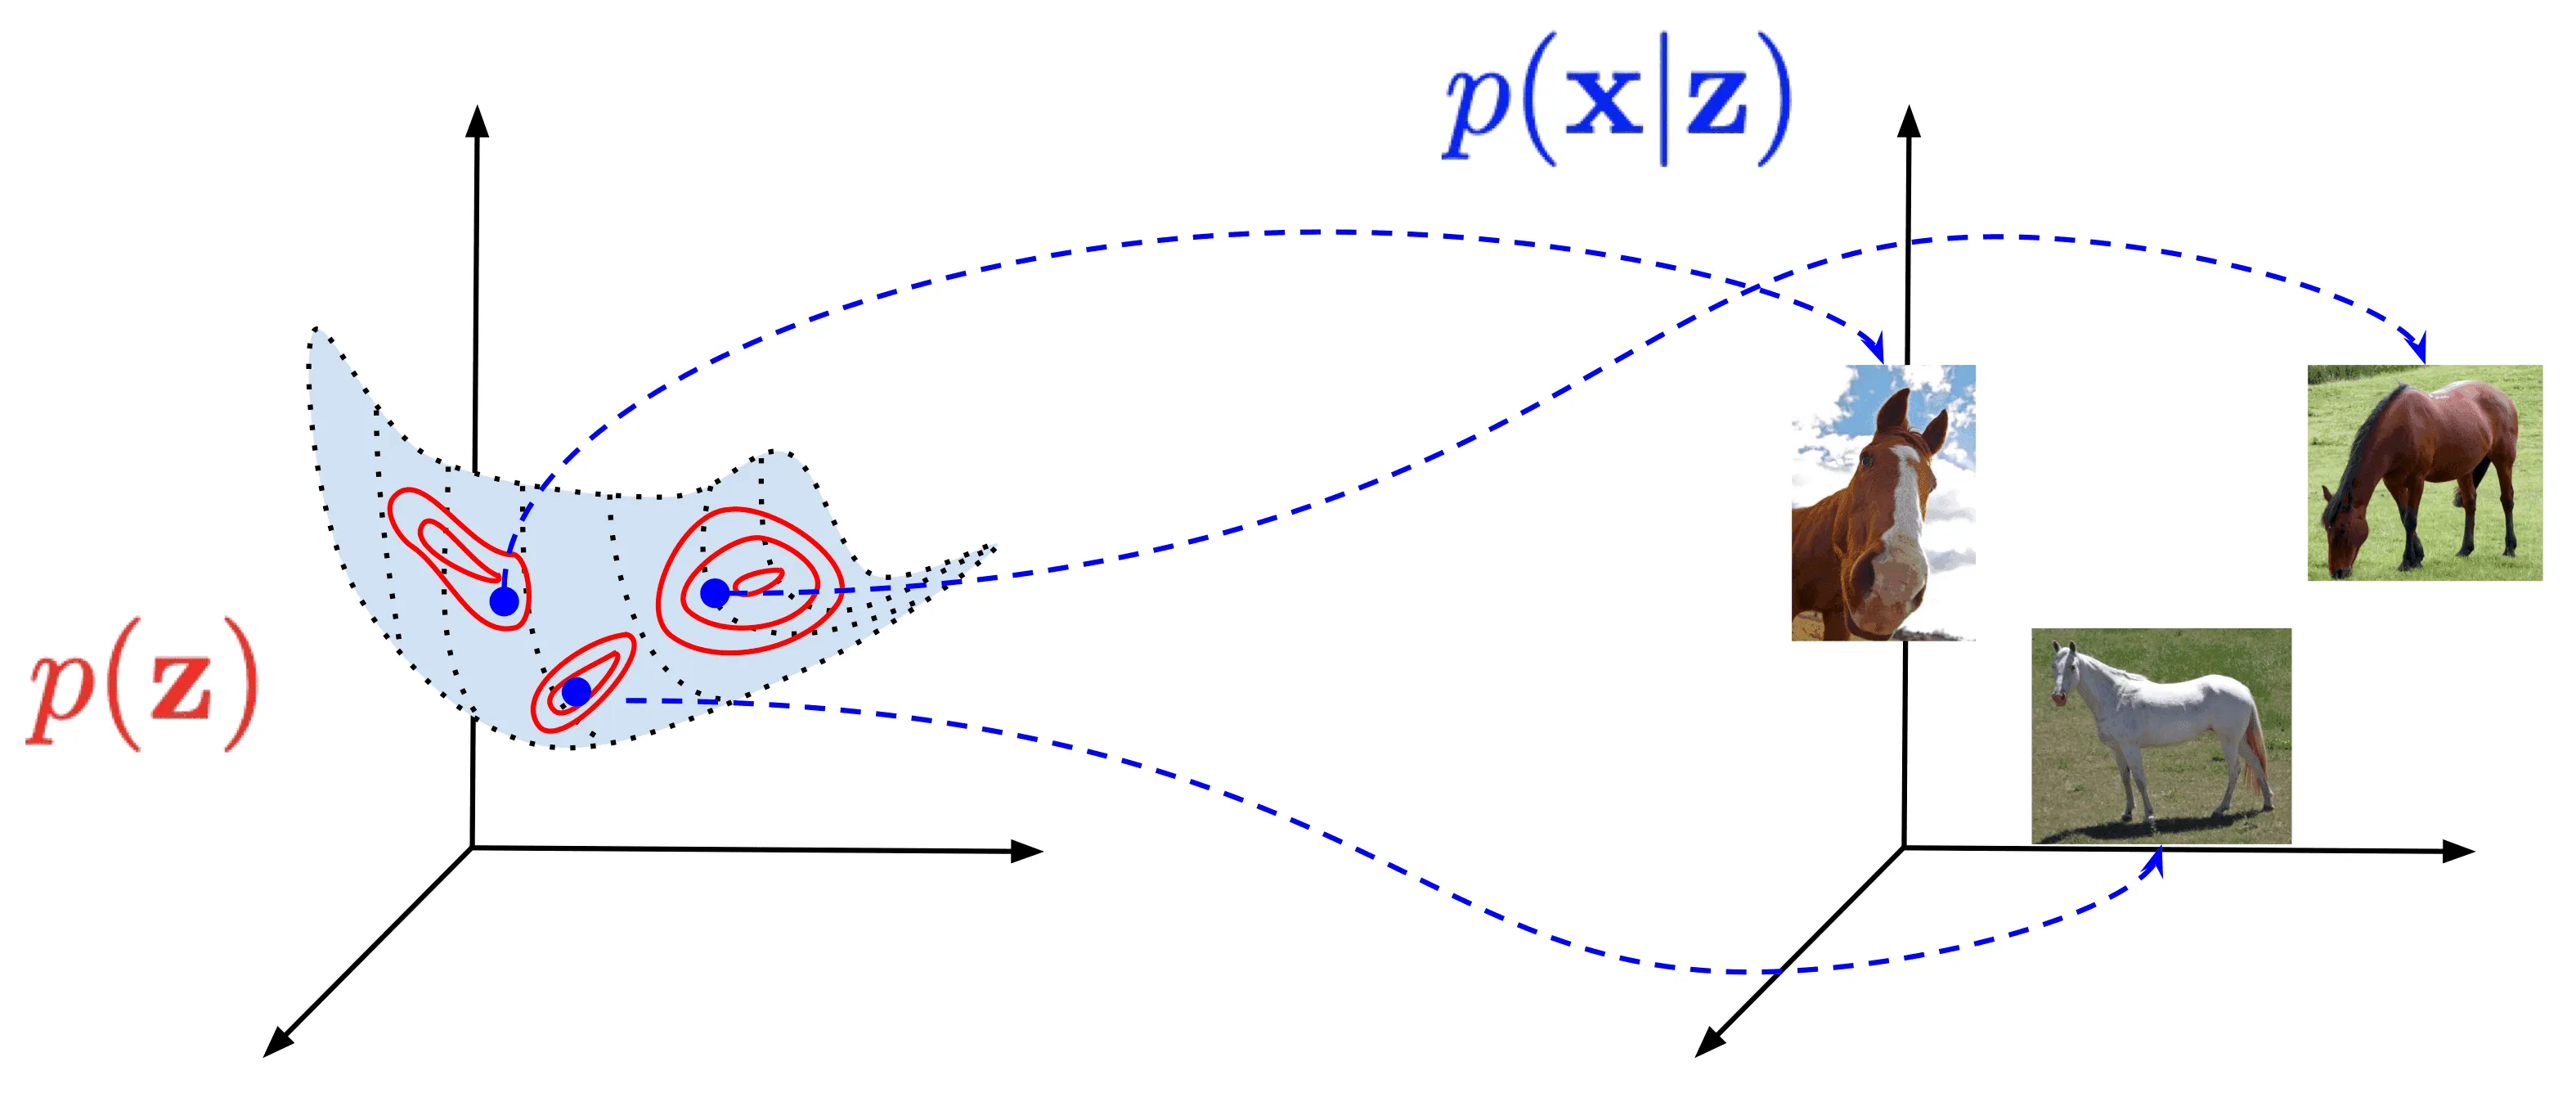
\includegraphics[width=.8\textwidth]{../resources/vae/sampling.png}
    \end{figure}
\end{frame}

\begin{frame}[allowframebreaks]{Интуиция}
    \textbf{Идея:}
    \begin{itemize}
        \item $f_{\boldsymbol{\theta}}(\boldsymbol{x}) = \boldsymbol{\psi}_{\boldsymbol{x}} = \left(\boldsymbol{\mu}_{\boldsymbol{x}}, \boldsymbol{\sigma}_{\boldsymbol{x}}^2\right)$ — параметры нормального распределения.
        \item $\boldsymbol{z} \sim p(\boldsymbol{z} \mid \boldsymbol{\psi}_{\boldsymbol{x}}) = \mathcal{N}(\boldsymbol{z} \mid \boldsymbol{\mu}_{\boldsymbol{x}}, \boldsymbol{\sigma}_{\boldsymbol{x}}^2)$.
        \item $\tilde{\boldsymbol{x}} = g_{\boldsymbol{\phi}}(\boldsymbol{z}) \sim p(\boldsymbol{x} \mid \boldsymbol{z})$.
    \end{itemize}

    \textbf{Параметры:}
    \begin{align*}
        \boldsymbol{\mu}_{\boldsymbol{x}}      & = \begin{bmatrix} \mu_{\boldsymbol{x}1} & \mu_{\boldsymbol{x}2} & \ldots & \mu_{\boldsymbol{x}M} \end{bmatrix},                                                \\
        \boldsymbol{\sigma}_{\boldsymbol{x}}^2 & = \operatorname{diag}\left(\begin{bmatrix} \sigma_{\boldsymbol{x}1}^2 & \sigma_{\boldsymbol{x}2}^2 & \ldots & \sigma_{\boldsymbol{x}M}^2 \end{bmatrix}\right).
    \end{align*}

    \framebreak

    \textbf{Проблемы:}
    \begin{enumerate}
        \item \textbf{Проблема 1:} модель стремится к $\boldsymbol{\sigma}_{\boldsymbol{x}}^2 = \mathbf{0}$, что превращает VAE в AE.
              \begin{itemize}
                  \item \textbf{Решение:} добавить регуляризационный член (какой?):
                        \begin{equation*}
                            \mathcal{L}(\boldsymbol{\theta}, \boldsymbol{\phi}) = \text{L}_{\text{rec}} + \alpha \text{L}_{\text{reg}}.
                        \end{equation*}
              \end{itemize}
        \item \textbf{Проблема 2:} сэмплирование не дифференцируемо.
    \end{enumerate}
\end{frame}

\begin{frame}{Правдоподобие $p(\boldsymbol{x})$}
    \textbf{Совместное распределение:}
    \begin{equation*}
        p_{\phi}(\boldsymbol{x}, \boldsymbol{z}) = p(\boldsymbol{x}, \boldsymbol{z} \mid \phi).
    \end{equation*}

    \textbf{Правдоподобие данных:}
    \begin{align*}
         & L(\phi) = \prod_{i=1}^N p_{\phi}(\boldsymbol{x}_i),          \\
         & \log L(\phi) = \sum_{i=1}^N \log p_{\phi}(\boldsymbol{x}_i).
    \end{align*}

    \textbf{Цель:} Максимизация правдоподобия:
    \begin{equation*}
        p_{\phi}(\boldsymbol{x}) = \int_{\boldsymbol{z}} p_{\phi}(\boldsymbol{x}, \boldsymbol{z}) d\boldsymbol{z} \to \max_{\phi \in \Phi}.
    \end{equation*}
\end{frame}

\begin{frame}[allowframebreaks]{Аппроксимация $p(\boldsymbol{z} \mid \boldsymbol{x})$}
    \textbf{Теорема Байеса:}
    \begin{equation*}
        p(\boldsymbol{z} \mid \boldsymbol{x}) = \frac{p(\boldsymbol{x}, \boldsymbol{z})}{p(\boldsymbol{x})} = \frac{p(\boldsymbol{x} \mid \boldsymbol{z}) p(\boldsymbol{z})}{p(\boldsymbol{x})}.
    \end{equation*}

    \textbf{Распределения:}
    \begin{itemize}
        \item $p(\boldsymbol{x})$: априорное распределение данных.
        \item $p(\boldsymbol{z} \mid \boldsymbol{x})$: распределение энкодера.
        \item $p(\boldsymbol{z}) = \mathcal{N}(\boldsymbol{z} \mid \mathbf{0}, \mathbf{E})$: априорное распределение латентного пространства.
        \item $p(\boldsymbol{x} \mid \boldsymbol{z}) \left(= \mathcal{N}(\boldsymbol{x} \mid g_{\boldsymbol{\phi}}(\boldsymbol{z}), c\mathbf{I})\right)$: распределение декодера.
    \end{itemize}

    \framebreak

    \textbf{Проблема:} $p(\boldsymbol{z} \mid \boldsymbol{x})$ имеет сложную форму:
    \begin{equation*}
        p(\boldsymbol{z} \mid \boldsymbol{x}) = \frac{\mathcal{N}(\boldsymbol{x} \mid g_{\boldsymbol{\phi}}(\boldsymbol{z}), c\mathbf{I}) \mathcal{N}(\boldsymbol{z} \mid \mathbf{0}, \mathbf{E})}{p(\boldsymbol{x})}.
    \end{equation*}

    \textbf{Workaround:} Аппроксимация через простое распределение $q(\boldsymbol{z})$:
    \begin{equation*}
        p(\boldsymbol{z} \mid \boldsymbol{x}) \approx q(\boldsymbol{z}) = \mathcal{N}(\boldsymbol{z} \mid \boldsymbol{\mu}_{\boldsymbol{x}}, \boldsymbol{\sigma}_{\boldsymbol{x}}^2).
    \end{equation*}
\end{frame}

\begin{frame}[allowframebreaks]{Вариационное приближение}
    \textbf{Цель:} Максимизировать правдоподобие $p(\boldsymbol{x})$:
    \begin{align*}
        \log p(\boldsymbol{x}) & = \log \int_{\boldsymbol{z}} p(\boldsymbol{x}, \boldsymbol{z})d\boldsymbol{z}  = \log \int_{\boldsymbol{z}} p(\boldsymbol{x} \mid \boldsymbol{z})p(\boldsymbol{z})d\boldsymbol{z} \\
                               & = \log \mathbb{E}_{q(\boldsymbol{z})}\left[\frac{p(\boldsymbol{z})p(\boldsymbol{x} \mid \boldsymbol{z})}{q(\boldsymbol{z})}\right].
    \end{align*}

    \textbf{Неравенства Йенсена:}
    \begin{align*}
         & g(\mathbb{E}[\xi]) \leq \mathbb{E}[g(\xi)], \quad g(x) \text{ \textemdash{} вогнутая функция}, \\
         & g(\mathbb{E}[\xi]) \geq \mathbb{E}[g(\xi)], \quad g(x) \text{ \textemdash{} выпуклая функция}.
    \end{align*}
    Применим к $\log$:
    \begin{align*}
        \log p(\boldsymbol{x}) & = \log \mathbb{E}_{q(\boldsymbol{z})}\left[\frac{p(\boldsymbol{z})p(\boldsymbol{x} \mid \boldsymbol{z})}{q(\boldsymbol{z})}\right] \geq \mathbb{E}_{q(\boldsymbol{z})}\left[\log \frac{p(\boldsymbol{z})p(\boldsymbol{x} \mid \boldsymbol{z})}{q(\boldsymbol{z})}\right] \\
                               & = \mathbb{E}_{q(\boldsymbol{z})}\left[\log p(\boldsymbol{x} \mid \boldsymbol{z})\right] - \mathbb{E}_{q(\boldsymbol{z})}\left[\log \frac{q(\boldsymbol{z})}{p(\boldsymbol{z})}\right]                                                                                    \\
                               & = \mathbb{E}_{q(\boldsymbol{z})}\left[\log p(\boldsymbol{x} \mid \boldsymbol{z})\right] - \text{KL}(q(\boldsymbol{z}) \parallel p(\boldsymbol{z})),
    \end{align*}
    где $\text{KL}$ — дивергенция Кульбака-Лейблера.

    \textbf{Итог:} Нижняя граница на $\log p(\boldsymbol{x})$ (Evidence Lower Bound, \textit{ELBO}):
    \begin{align*}
        \log p(\boldsymbol{x}) \geq \mathbb{E}_{q(\boldsymbol{z})}\left[\log p(\boldsymbol{x} \mid \boldsymbol{z})\right] - \text{KL}(q(\boldsymbol{z}) \parallel p(\boldsymbol{z})) \to \max_{q(\boldsymbol{z})}.
    \end{align*}
\end{frame}

\begin{frame}{Распределение $p(\boldsymbol{x} \mid \boldsymbol{z})$}
    $p(\boldsymbol{x} \mid \boldsymbol{z}) = \mathcal{N}(\boldsymbol{x} \mid g_{\boldsymbol{\phi}}(\boldsymbol{z}), c\mathbf{I})$, $c \neq 0$, поэтому матрица ковариации невырождена.

    \begin{align*}
        p(\boldsymbol{x} \mid \boldsymbol{z})
         & = \frac{1}{(2\pi)^{D/2}|c\mathbf{I}|^{1/2}}\exp\left(-\frac{1}{2}(\boldsymbol{x} - g_{\boldsymbol{\phi}}(\boldsymbol{z}))^T(c\mathbf{I})^{-1}(\boldsymbol{x} - g_{\boldsymbol{\phi}}(\boldsymbol{z}))\right) \\
         & = \frac{1}{(2\pi)^{D/2}c^{D/2}}\exp\left(-\frac{1}{2c}\|\boldsymbol{x} - g_{\boldsymbol{\phi}}(\boldsymbol{z})\|^2_2\right)                                                                                  \\
         \\
        \log(p(\boldsymbol{x} \mid \boldsymbol{z}))
         & = -\frac{D}{2}\log(2\pi) - \frac{D}{2}\log(c) - \frac{1}{2c}\|\boldsymbol{x} - g_{\boldsymbol{\phi}}(\boldsymbol{z})\|^2_2                                                                                   \\
         & = \text{const} - \frac{1}{2c}\|\boldsymbol{x} - g_{\boldsymbol{\phi}}(\boldsymbol{z})\|^2_2.
    \end{align*}
\end{frame}

\begin{frame}{Итоговая оптимизация}
    \textbf{Оптимизационная задача:}
    \begin{align*}
         & \mathbb{E}_{q(\boldsymbol{z})}\left[\log p(\boldsymbol{x} \mid \boldsymbol{z})\right] - \text{KL}(q(\boldsymbol{z}) \parallel p(\boldsymbol{z}))                                                                  \\
         & = -\mathbb{E}_{q(\boldsymbol{z})}\left[\frac{1}{2c}\|\boldsymbol{x} - g_{\boldsymbol{\phi}}(\boldsymbol{z})\|^2_2\right] - \text{KL}(q(\boldsymbol{z}) \parallel p(\boldsymbol{z})) \to \max_{q(\boldsymbol{z})}.
    \end{align*}

    \textbf{Эквивалентная формулировка:}
    \begin{align*}
         & \mathbb{E}_{q(\boldsymbol{z})}\left[\frac{1}{2c}\|\boldsymbol{x} - g_{\boldsymbol{\phi}}(\boldsymbol{z})\|^2_2\right] + \text{KL}(q(\boldsymbol{z}) \parallel p(\boldsymbol{z})) \to \min_{q(\boldsymbol{z})}.
    \end{align*}
\end{frame}

\begin{frame}{Вспомним интуицию}
    \textbf{Получили то, чего и хотели:}
    \begin{align*}
        \text{L}_{\text{rec}} & = \frac{1}{2c}\|\boldsymbol{x} - g_{\boldsymbol{\phi}}(\boldsymbol{z})\|^2_2, \\
        \text{L}_{\text{reg}} & = \text{KL}(q(\boldsymbol{z}) \parallel p(\boldsymbol{z})).
    \end{align*}

    \textbf{Итог:}
    Баланс между реконструкцией данных и отклонением от априорного распределения в латентном пространстве.
\end{frame}

\begin{frame}[allowframebreaks]{Вычисление $\text{L}_{\text{reg}}$}
    \begin{align*}
        & \text{KL}(q(\boldsymbol{z}) \parallel p(\boldsymbol{z})) = \text{KL}\left(\boldsymbol{\mathcal{N}}(\boldsymbol{z} \mid \boldsymbol{\mu}_{\boldsymbol{x}}, \boldsymbol{\sigma}_{\boldsymbol{x}}^2) \parallel \boldsymbol{\mathcal{N}}(\boldsymbol{z} \mid \mathbf{0}, \mathbf{E})\right) \\
        &= \text{KL}\left(\prod_{i=1}^M\boldsymbol{\mathcal{N}}(z_i \mid \mu_{\boldsymbol{x}i}, \sigma_{\boldsymbol{x}i}^2) \parallel \prod_{i=1}^M\boldsymbol{\mathcal{N}}(z_i \mid 0, 1)\right) = \text{KL}\left(\prod_{i=1}^Mq_i(\boldsymbol{z}_i) \parallel \prod_{i=1}^Mp_i(\boldsymbol{z}_i)\right) \\
        &= \int_{\boldsymbol{z}} \prod_{i=1}^Mq_i(\boldsymbol{z}_i)\log\frac{\prod_{i=1}^Mq_i(\boldsymbol{z}_i)}{\prod_{i=1}^Mp_i(\boldsymbol{z}_i)}d\boldsymbol{z} = \int_{\boldsymbol{z}} \prod_{i=1}^Mq_i(\boldsymbol{z}_i)\left(\sum_{i=1}^M\log \frac{q_i(\boldsymbol{z}_i)}{p_i(\boldsymbol{z}_i)}\right)d\boldsymbol{z} \\
        &= \sum_{j=1}^M\int_{\boldsymbol{z}} \log \frac{q_j(\boldsymbol{z}_j)}{p_j(\boldsymbol{z}_j)} \prod_{i=1}^Mq_i(\boldsymbol{z}_i) d\boldsymbol{z}_1\ldots d\boldsymbol{z}_M \\
        &= \sum_{j=1}^M \left( \left( \int_{\boldsymbol{z}_j} \log \frac{q_j(\boldsymbol{z}_j)}{p_j(\boldsymbol{z}_j)}q_j(\boldsymbol{z}_j) d\boldsymbol{z}_j \right) \prod_{i\neq j}^M \int_{\boldsymbol{z}_i} q_i(\boldsymbol{z}_i) d\boldsymbol{z}_i \right) = \ldots
    \end{align*}

    \begin{align*}
        &= \sum_{j=1}^M \left( \int_{\boldsymbol{z}_j} \log \frac{q_j(\boldsymbol{z}_j)}{p_j(\boldsymbol{z}_j)}q_j(\boldsymbol{z}_j) d\boldsymbol{z}_j \right) = \sum_{j=1}^M \text{KL}(q_j(\boldsymbol{z}_j) \parallel p_j(\boldsymbol{z}_j))
    \end{align*}

    \textbf{Для каждой компоненты:}
    \begin{align*}
        \text{KL}(q_j(\boldsymbol{z}_j) \parallel p_j(\boldsymbol{z}_j)) &= \int_{z_j} \mathcal{N}(z_j \mid \mu_{\boldsymbol{x}j}, \sigma_{\boldsymbol{x}j}^2) \log \frac{\mathcal{N}(z_j \mid \mu_{\boldsymbol{x}j}, \sigma_{\boldsymbol{x}j}^2)}{\mathcal{N}(z_j \mid 0, 1)} dz_j.\\
        &= \mathbb{E}_{q_j(z_j)}\left[\log \mathcal{N}(z_j \mid \mu_{\boldsymbol{x}j}, \sigma_{\boldsymbol{x}j}^2) - \log \mathcal{N}(z_j \mid 0, 1)\right].
    \end{align*}

    \textbf{Распределение $\mathcal{N}$:}
    \begin{align*}
        \log \mathcal{N}(z_j \mid \mu_{\boldsymbol{x}j}, \sigma_{\boldsymbol{x}j}^2) &= -\frac{1}{2}\log(2\pi\sigma_{\boldsymbol{x}j}^2) - \frac{1}{2\sigma_{\boldsymbol{x}j}^2}(z_j - \mu_{\boldsymbol{x}j})^2, \\
        \log \mathcal{N}(z_j \mid 0, 1) &= -\frac{1}{2}\log(2\pi) - \frac{1}{2}z_j^2.
    \end{align*}
    \textbf{Разница логарифмов:}
    \begin{align*}
        \log \mathcal{N}(z_j \mid \mu_{\boldsymbol{x}j}, \sigma_{\boldsymbol{x}j}^2) - \log \mathcal{N}(z_j \mid 0, 1) &= -\frac{1}{2}\log(\sigma_{\boldsymbol{x}j}^2) - \frac{1}{2\sigma_{\boldsymbol{x}j}^2}(z_j - \mu_{\boldsymbol{x}j})^2 + \frac{1}{2}z_j^2.
    \end{align*}

    \textbf{Итоговая формула:}
    \begin{align*}
        & \text{KL}(q_j(\boldsymbol{z}_j) \parallel p_j(\boldsymbol{z}_j)) = \mathbb{E}_{q_j(z_j)}\left[-\frac{1}{2}\log(\sigma_{\boldsymbol{x}j}^2) - \frac{1}{2\sigma_{\boldsymbol{x}j}^2}(z_j - \mu_{\boldsymbol{x}j})^2 + \frac{1}{2}z_j^2\right] \\
        &= \mathbb{E}_{q_j(z_j)}\left[ -\left(\frac{1}{2}\log(\sigma_{\boldsymbol{x}j}^2) + \frac{\mu_{\boldsymbol{x}j}^2}{2\sigma_{\boldsymbol{x}j}^2} \right) + \left(\frac{1}{2} - \frac{1}{2\sigma_{\boldsymbol{x}j}^2}\right)z_j^2 + \frac{\mu_{\boldsymbol{x}j}}{\sigma_{\boldsymbol{x}j}^2}z_j \right] \\
        &= -\left(\frac{1}{2}\log(\sigma_{\boldsymbol{x}j}^2) + \frac{\mu_{\boldsymbol{x}j}^2}{2\sigma_{\boldsymbol{x}j}^2} \right) + \left(\frac{1}{2} - \frac{1}{2\sigma_{\boldsymbol{x}j}^2}\right)\mathbb{E}_{q_j(z_j)}\left[z_j^2 \right] + \frac{\mu_{\boldsymbol{x}j}}{\sigma_{\boldsymbol{x}j}^2} \mathbb{E}_{q_j(z_j)}\left[z_j \right] = \ldots
    \end{align*}

    \textbf{Математические ожидания:}
    \begin{align*}
        & \mathbb{E}_{q_j(z_j)}\left[z_j \right] = \mu_{\boldsymbol{x}j}, \\
        & \mathbb{D}_{q_j(z_j)}\left[z_j \right] = \mathbb{E}_{q_j(z_j)}\left[z_j^2 \right] - \mu_{\boldsymbol{x}j}^2 = \sigma_{\boldsymbol{x}j}^2 \quad\Rightarrow\quad\mathbb{E}_{q_j(z_j)}\left[z_j^2 \right] = \sigma_{\boldsymbol{x}j}^2 + \mu_{\boldsymbol{x}j}^2.
    \end{align*}
    \textbf{Подстановка:}
    \begin{align*}
        \ldots 
        &= -\frac{1}{2}\log(\sigma_{\boldsymbol{x}j}^2) - \frac{\mu_{\boldsymbol{x}j}^2}{2\sigma_{\boldsymbol{x}j}^2} + \frac{1}{2}\left(1 - \frac{1}{\sigma_{\boldsymbol{x}j}^2}\right)(\sigma_{\boldsymbol{x}j}^2 + \mu_{\boldsymbol{x}j}^2) + \frac{\mu_{\boldsymbol{x}j}}{\sigma_{\boldsymbol{x}j}^2} \mu_{\boldsymbol{x}j} \\
        &= -\frac{1}{2}\log(\sigma_{\boldsymbol{x}j}^2) - \frac{\mu_{\boldsymbol{x}j}^2}{2\sigma_{\boldsymbol{x}j}^2} + \frac{1}{2}\left(\sigma_{\boldsymbol{x}j}^2 + \mu_{\boldsymbol{x}j}^2 - 1 - \frac{\mu_{\boldsymbol{x}j}^2}{\sigma_{\boldsymbol{x}j}^2} \right) + \frac{\mu_{\boldsymbol{x}j}^2}{\sigma_{\boldsymbol{x}j}^2} \\
        &= -\frac{1}{2}\log(\sigma_{\boldsymbol{x}j}^2) + \frac{1}{2}\sigma_{\boldsymbol{x}j}^2 + \frac{1}{2}\mu_{\boldsymbol{x}j}^2 - \frac{1}{2} \\
        &= \frac{1}{2}\left( \sigma_{\boldsymbol{x}j}^2 + \mu_{\boldsymbol{x}j}^2 - 1 - \log(\sigma_{\boldsymbol{x}j}^2) \right)
    \end{align*}
\end{frame}

\begin{frame}{Функционал потерь}
    \textbf{Итоговые формулы:}
    \begin{align*}
        \text{L}_{\text{rec}} &= \frac{1}{2c}\|\boldsymbol{x} - g_{\boldsymbol{\phi}}(\boldsymbol{z})\|^2_2, \\
        \text{L}_{\text{reg}} &= \sum_{j=1}^M \frac{1}{2}\left( \sigma_{\boldsymbol{x}j}^2 + \mu_{\boldsymbol{x}j}^2 - 1 - \log(\sigma_{\boldsymbol{x}j}^2) \right).
    \end{align*}
    \textbf{Дополнение:} Для $\text{L}_{\text{rec}}$ также можно использовать кросс-энтропию.
\end{frame}

\begin{frame}{Reparametrization trick}
    \begin{align*}
        \boldsymbol{z}_j &\sim \boldsymbol{\mathcal{N}}( \boldsymbol{z}_j \mid \mu_{\boldsymbol{x}j}, \sigma_{\boldsymbol{x}j}^2) \Leftrightarrow
        \begin{cases}
            & \boldsymbol{\varepsilon}_j \sim \boldsymbol{\mathcal{N}}(0, 1), \\
            & \boldsymbol{z}_j = \mu_{\boldsymbol{x}j} + \sigma_{\boldsymbol{x}j}\boldsymbol{\varepsilon}_j.
        \end{cases}
    \end{align*}

    \textbf{Поскольку:}
    \begin{align*}
        p_{\varepsilon}(\varepsilon) &= \frac{1}{\sqrt{2\pi}}\exp\left(-\frac{\varepsilon^2}{2}\right), \\
        \varepsilon &= \frac{z - \mu_{\boldsymbol{x}}}{\sigma_{\boldsymbol{x}}}, \quad \sigma_{\boldsymbol{x}} > 0, \\
        \left|\frac{d\varepsilon}{dz}\right| &= \frac{1}{\sigma_{\boldsymbol{x}}}, \\
        p_z(z) &= p_{\varepsilon}\left(\frac{z - \mu_{\boldsymbol{x}}}{\sigma_{\boldsymbol{x}}}\right)\left|\frac{d\varepsilon}{dz}\right| = \frac{1}{\sqrt{2\pi}\sigma_{\boldsymbol{x}}}\exp\left(-\frac{(z - \mu_{\boldsymbol{x}})^2}{2\sigma_{\boldsymbol{x}}^2}\right).
    \end{align*}
\end{frame}

\begin{frame}{Архитектура VAE}
    \begin{figure}
        \centering
        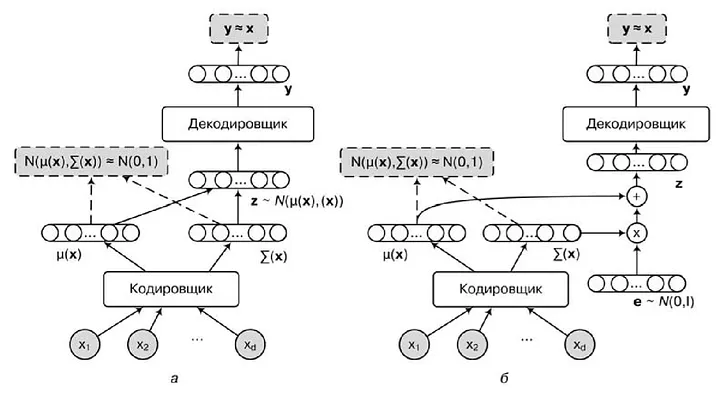
\includegraphics[width=1\textwidth]{../resources/vae/vae.png}
    \end{figure}
\end{frame}

\begin{frame}{Детали реализации}
    \textbf{Проблема:} $\forall i \quad 0 < \boldsymbol{\sigma}_{\boldsymbol{xi}}^2 \ll 1$ \textemdash{} маленькие значения могут приводить к ошибкам численных расчетов.

    \textbf{Решение:} Использовать логарифмированное значение $\boldsymbol{\sigma}_{\boldsymbol{xi}}^2$:
    \begin{equation*}
        \log \boldsymbol{\sigma}_{\boldsymbol{xi}}^2  \in \mathbb{R}^M.
    \end{equation*}

    \textbf{Репараметризация:}
    \begin{align*}
        \boldsymbol{\varepsilon}_j &\sim \boldsymbol{\mathcal{N}}(0, 1), \\
        \boldsymbol{z}_j &= \mu_{\boldsymbol{x}j} + \exp\left(\frac{1}{2}\log \boldsymbol{\sigma}_{\boldsymbol{xi}}^2 \right)\boldsymbol{\varepsilon}_j.
    \end{align*}
\end{frame}

\begin{frame}{Практика}
    \begin{figure}
        \centering
        
\includegraphics[width=.3\textwidth]{../resources/overall/Jupyter_logo.png}
    \end{figure}
\end{frame}


\section{Заключение}

\begin{frame}[allowframebreaks]{Сравнительный анализ методов: особенности применения}
    \textbf{Ключевые отличия:}
    \begin{itemize}
        \item \textbf{PCA:} базовый линейный метод, идеален для анализа небольших и линейных зависимостей. Часто используется для визуализации и как отправная точка в анализе данных.
        \item \textbf{KPCA:} позволяет работать с нелинейной структурой данных, но требует осторожного выбора ядерной функции и гиперпараметров. Идеален для задач распознавания образов и биоинформатики.
        \item \textbf{AE:} предоставляет большую гибкость благодаря нейронным сетям. Находит применение в обработке данных и сложных задачах анализа.
        \item \textbf{VAE:} расширяет автоэнкодеры за счет вероятностной модели, идеально подходит для задач генерации данных и анализа латентных переменных.
    \end{itemize}
    \textbf{Дополнительно:}
    \begin{itemize}
        \item Все методы обладают уникальными преимуществами и ограничениями, что делает их подходящими для разных классов задач.
        \item Выбор метода зависит от структуры данных, целей анализа и доступных вычислительных ресурсов.
    \end{itemize}
\end{frame}

\begin{frame}[allowframebreaks]{Заключение}
    \textbf{Современные вызовы:} Работа с высокоразмерными данными требует гибких и мощных инструментов.

    \textbf{Основные итоги:}
    \begin{itemize}
        \item \textbf{Линейные методы} (например, PCA) остаются незаменимыми благодаря своей простоте и эффективности.
        \item \textbf{Нелинейные подходы}, такие как KPCA, открывают возможности работы с более сложными структурами данных.
        \item \textbf{Автоэнкодеры} обеспечивают исключительную гибкость для задач генерации данных и анализа скрытых зависимостей.
    \end{itemize}

    \framebreak

    \textbf{Рекомендации по выбору:}
    \begin{itemize}
        \item Для интерпретируемости и быстродействия – линейные методы.
        \item Для работы с нелинейными структурами – Kernel PCA.
        \item Для генерации данных – автоэнкодеры и их вариации.
    \end{itemize}

    \textbf{Вывод:} Методы понижения размерности предоставляют исследователям мощный арсенал для анализа данных, повышая информативность, эффективность и удобство визуализации.
\end{frame}


\end{document}
